\section{Performance Evaluation}
We use Omnet++(5.6.2) as the primary network simulation platform and evaluate the performance of our method and SPF[2] in terms of packet delivery ratio, link utilization, times of dropping packets, occupying ratio of the queue, remaining battery, and end-to-end delay in the satellite network whose constellation type is Walker[3].

\subsection{Simulation Parameters}
The simulation parameters are shown in \ref{table:PARAMETERS}. Each satellite is assumed to have four ISLs with two intra-orbits ISLs and two inter-orbits ISLs. The packet size is fixed to 1000 bits. In each packet transmission, it will cost 0.7 joules on transmitter satellite and 0.4 joules on receiver satellite per packet. The number, the source, and the destination of packets will be generated randomly based on the population distribution \cite{TRAFFICDENSITY}.

\begin{table*}[h]
	\caption{Simulation Parameters}
	\label{table:PARAMETERS}
\begin{center}
\begin{tabular}{|l|l|}
\hline
\textbf{Parameters} & \textbf{Values}           \\  \hline
Constellation type            & Walker          \\ \hline
Orbital height                & 780 km          \\ \hline
Number of orbital planes      & 6               \\ \hline
Number of satellites in orbit & 11              \\ \hline
Orbital inclination           & 86.4°           \\ \hline
Packet size                   & 1000 bits       \\ \hline
Initial battery energy        & 5000 joules     \\ \hline
Transmission required energy  & 0.7  joules     \\ \hline
Reception required energy     & 0.4  joules     \\ \hline
$\alpha$                      & 0.5             \\ \hline
$T_{dre}$                     & 0.06 ms       \\ \hline
\end{tabular}
\end{center}
\end{table*}

\subsection{Impact of Queue Size}
We first evaluate the relationship between queue length of the receiver satellite and the packet delivery ratio. The channel data rate is 10Mbps, and the unit of the queue is one packet (i.e., 1000 bits). \ref{fig:QUEDELIVERY} shows the delivery ratio for the examined schemes and various queue length. We can see both delivery ratios of the two schemes rise with the increased length of the queue since the packet has a longer time to keep in the queue and be processed. However, the growth rate of DEAL is higher than SPF's. This is because in DEAL, we split the traffic flow to avoid congestion, i.e., avoid sending all packets with the same link/path.  The modeling results suggest that DEAL achieves lower queue lengths than SPF.

To observe the probability of congestion and the pressure of queue, we evaluate the mean occupying ratio of two schemes. \ref{fig:QUEOCCUPYING} shows the mean occupying ratio of the queue with various queue length. Clearly, the higher the occupying ratio of a queue is, the higher the probability of dropping a packet is. 

\begin{figure}[htp]
	\centering
	\subfigure[]{
		\centering
		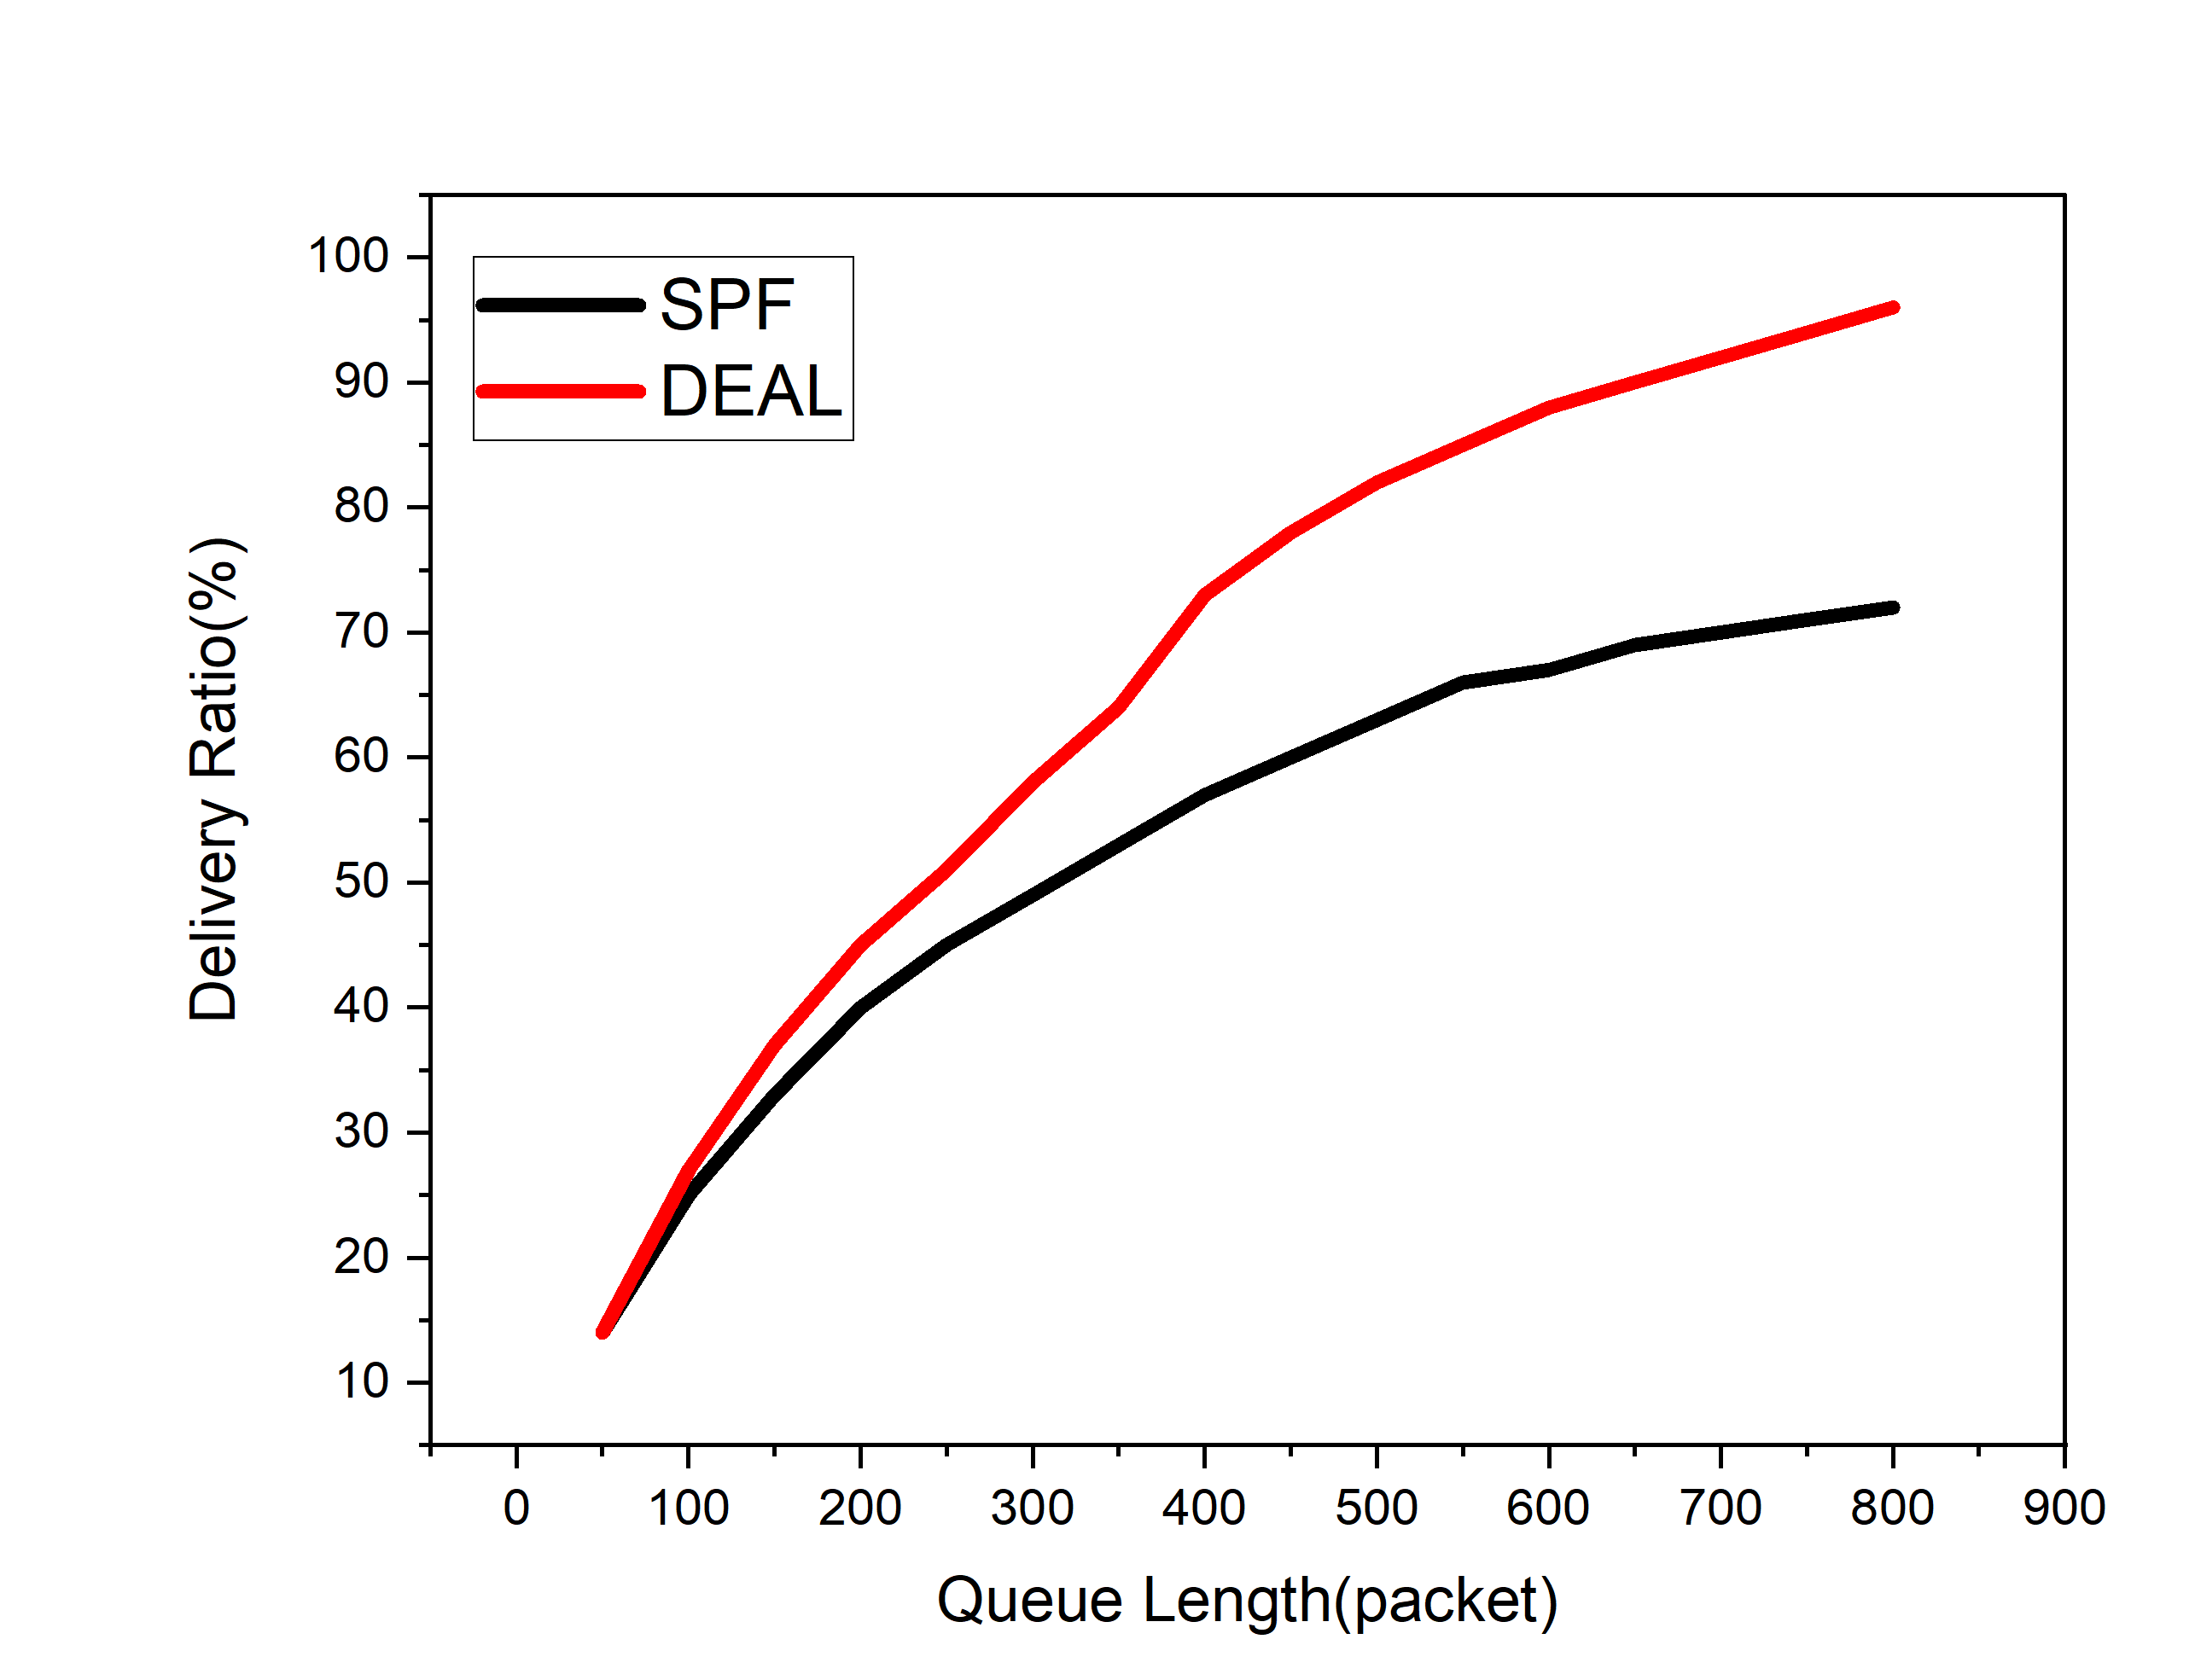
\includegraphics[width=.8\linewidth]{fig/simulation/queue/Queue-Delivery.png}
		\label{fig:QUEDELIVERY}
		}
	\subfigure[]{
		\centering
		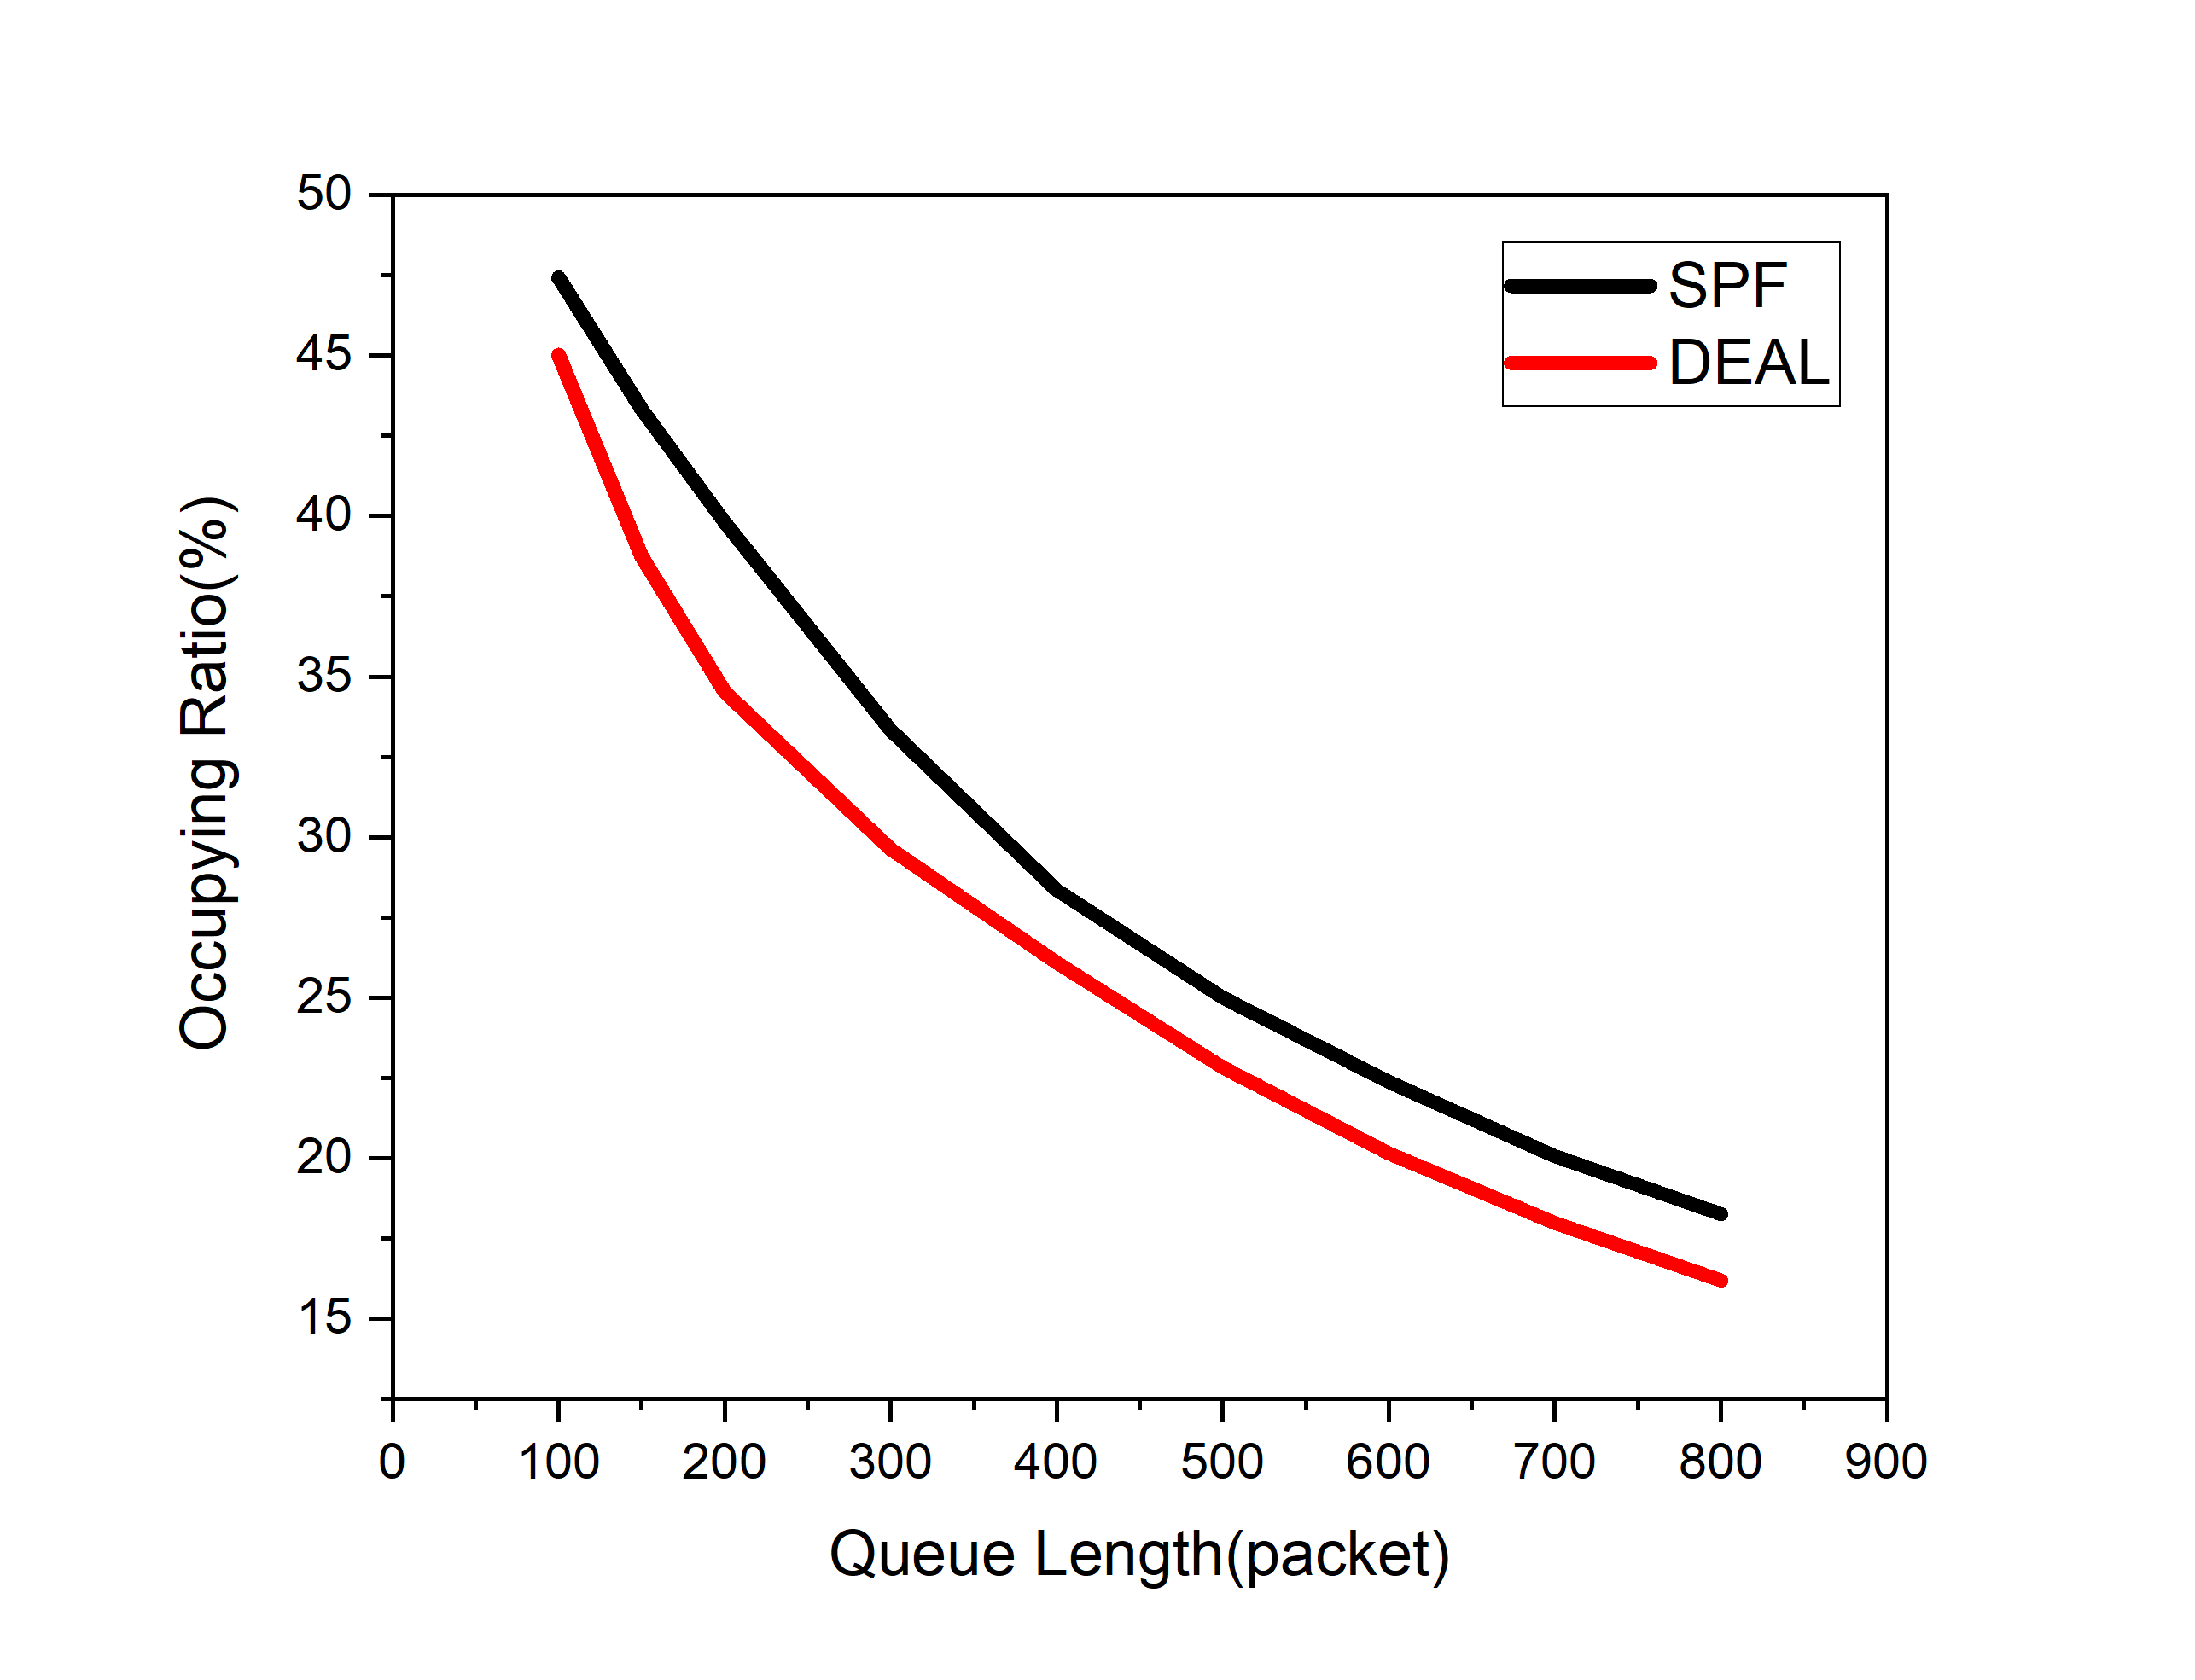
\includegraphics[width=.9\linewidth]{fig/simulation/queue/Queue-Occupying.png}
		\label{fig:QUEOCCUPYING}
		}
\caption{ (a) Delivery ratio with different buffer queue length (b) Mean Occupying ratio with different buffer queue length}
\label{fig:QUEUE}
\end{figure}

The number of dropped packets of each satellite is shown in \ref{fig:DROPPEDPACKETS}. We first labelled all the satellites as 2-digit number. The number of dropped packets in is extremely high in specific satellites because they are covering large-traffic areas, e.g. the U.S.A, China.  \ref{fig:DROPPEDPACKETSCDF} shows the CDF of dropped packets, the probability of dropped more than 40 packets is more than  10\%  in  SPF but less than 6\% in DEAL.  The performance of DEAL is better than SPF because the congestion level in  SPF is more severe. This is because our scheme  achieve a higher delivery ratio (under the same queue size) and lower the burden of queues on average. Moreover, with small queue size, the satellite in our scheme can save precious memory on satellite.
\begin{equation}
  Occupying\ Ratio\ of\ Queue :  \frac{\text { packet number in queue }}{\text { capacity of queue }} 
\end{equation}

\begin{figure}[htp]
	\subfigure[]{
		\centering
		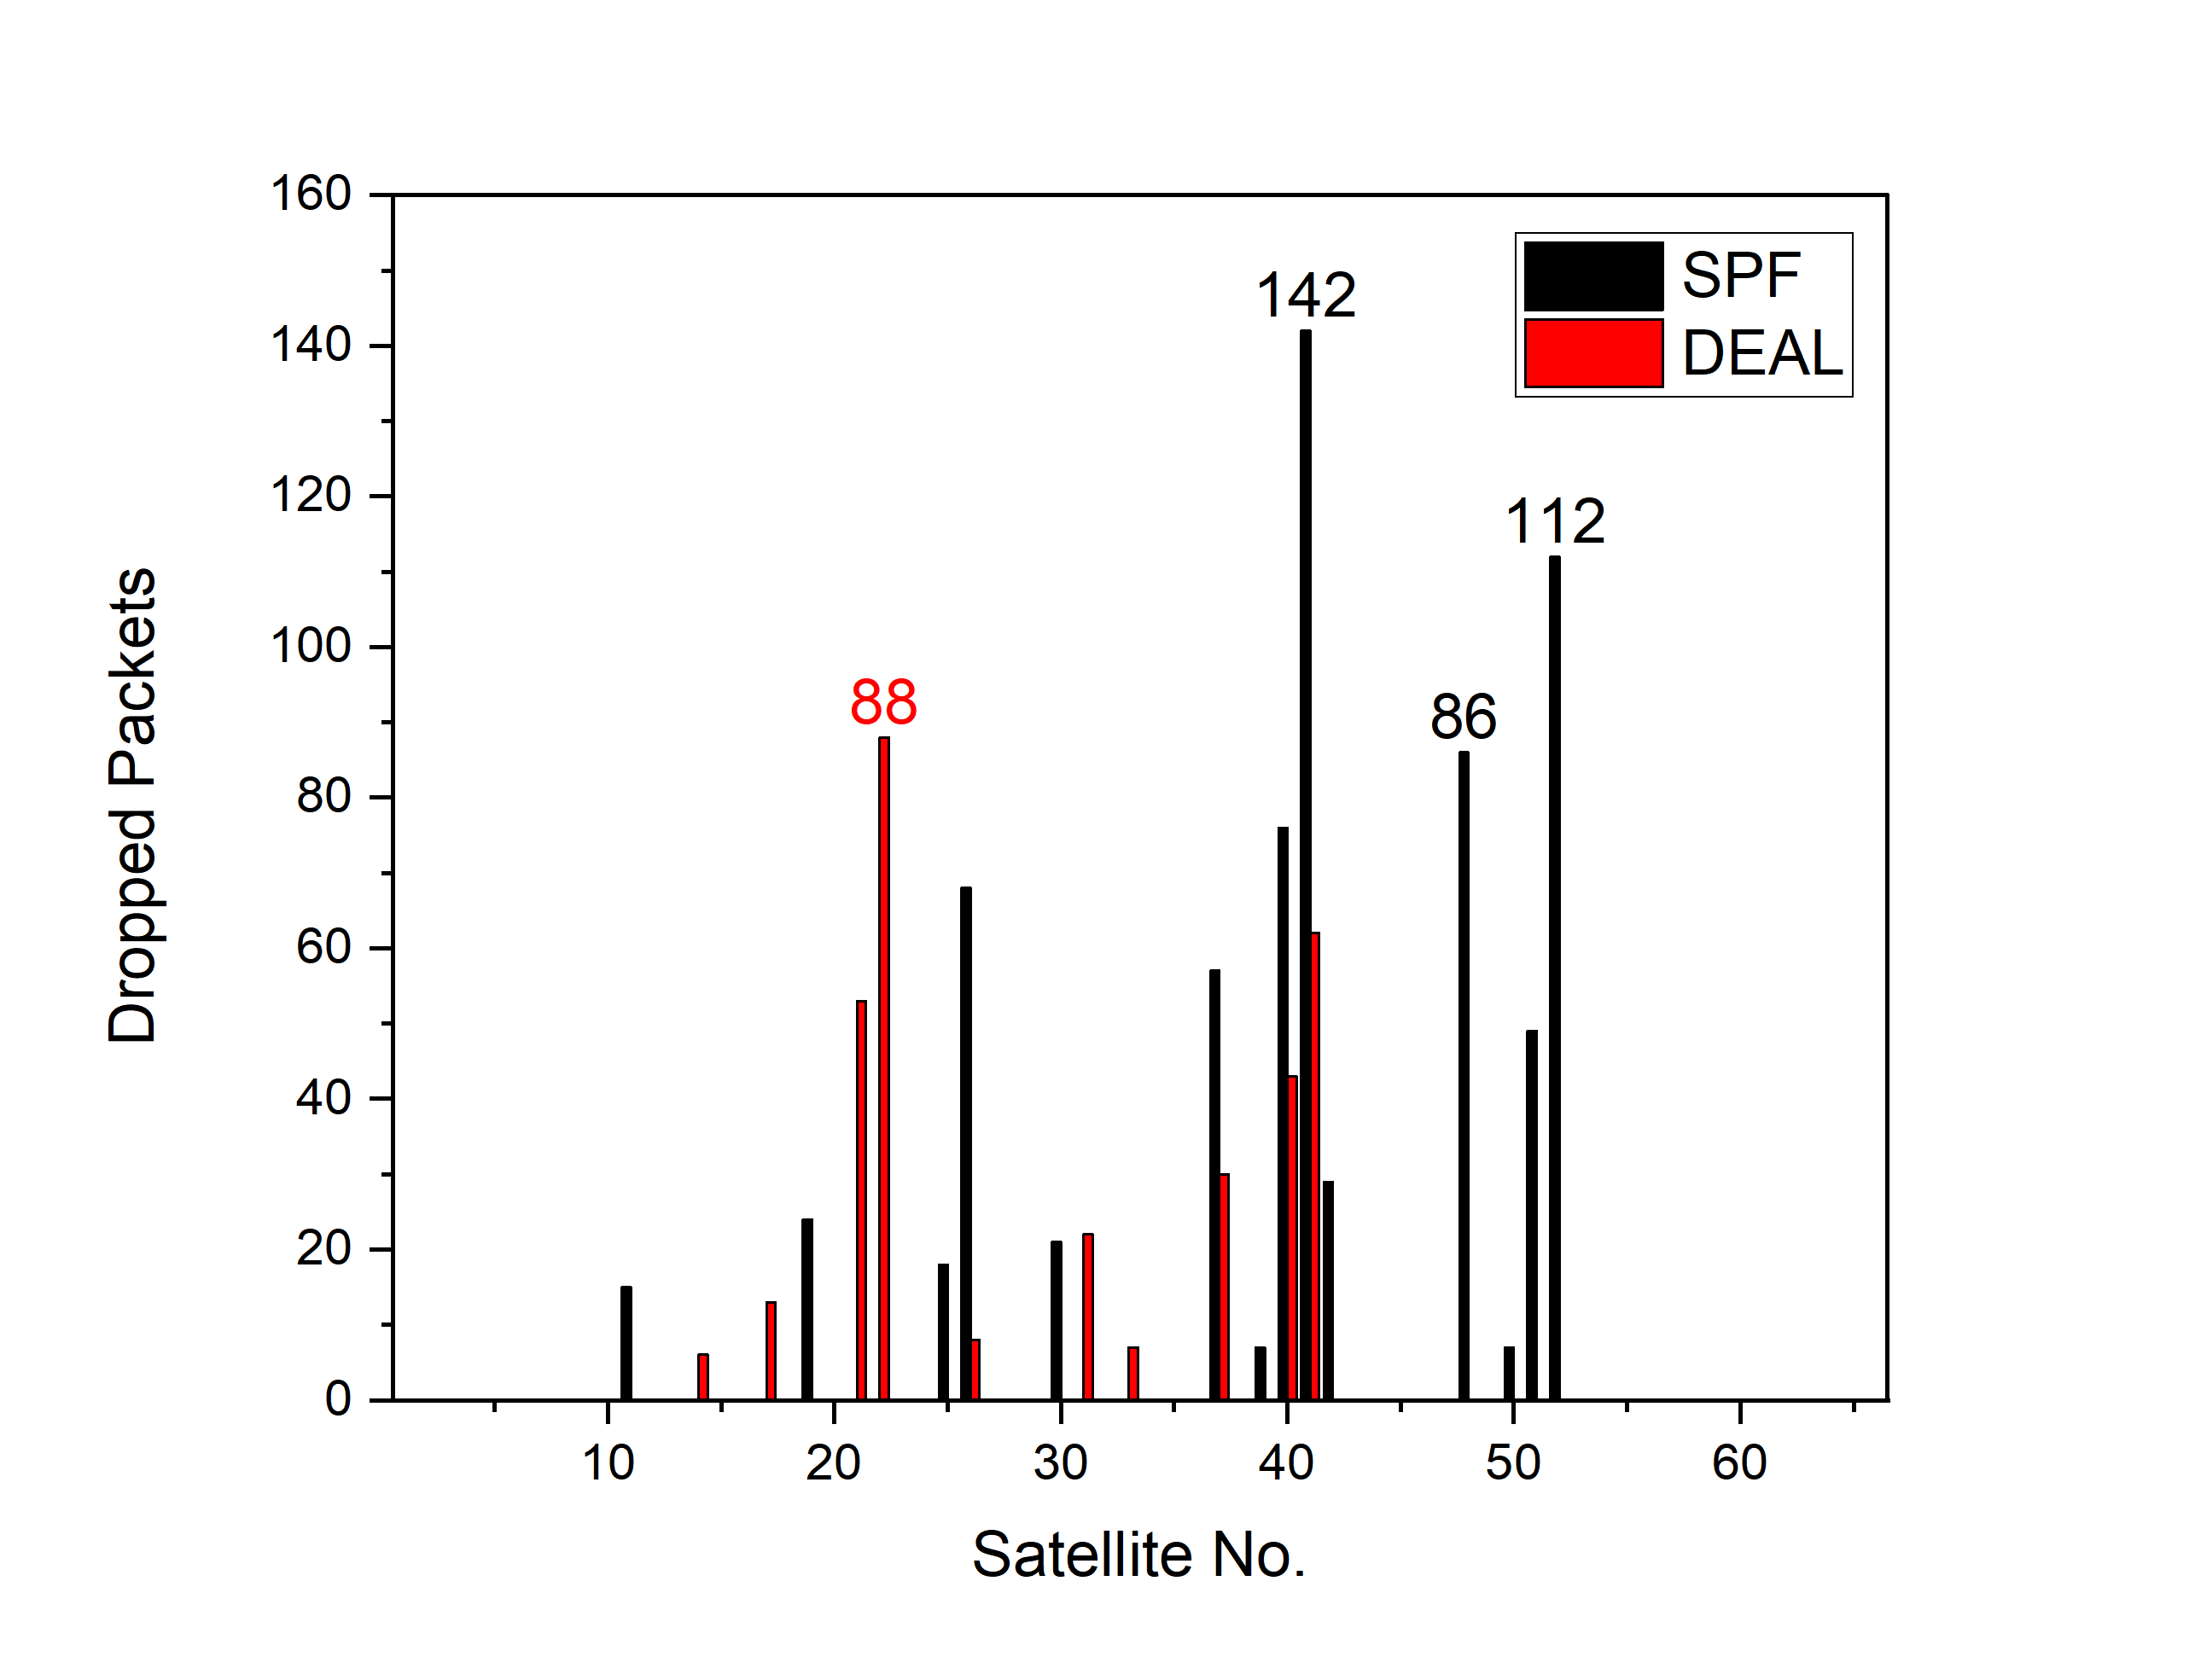
\includegraphics[width=.8\linewidth]{fig/simulation/droppedpacket/DroppedPacketsNumber.png}
		\label{fig:DROPPEDPACKETS}
		}
	\subfigure[]{
		\centering
		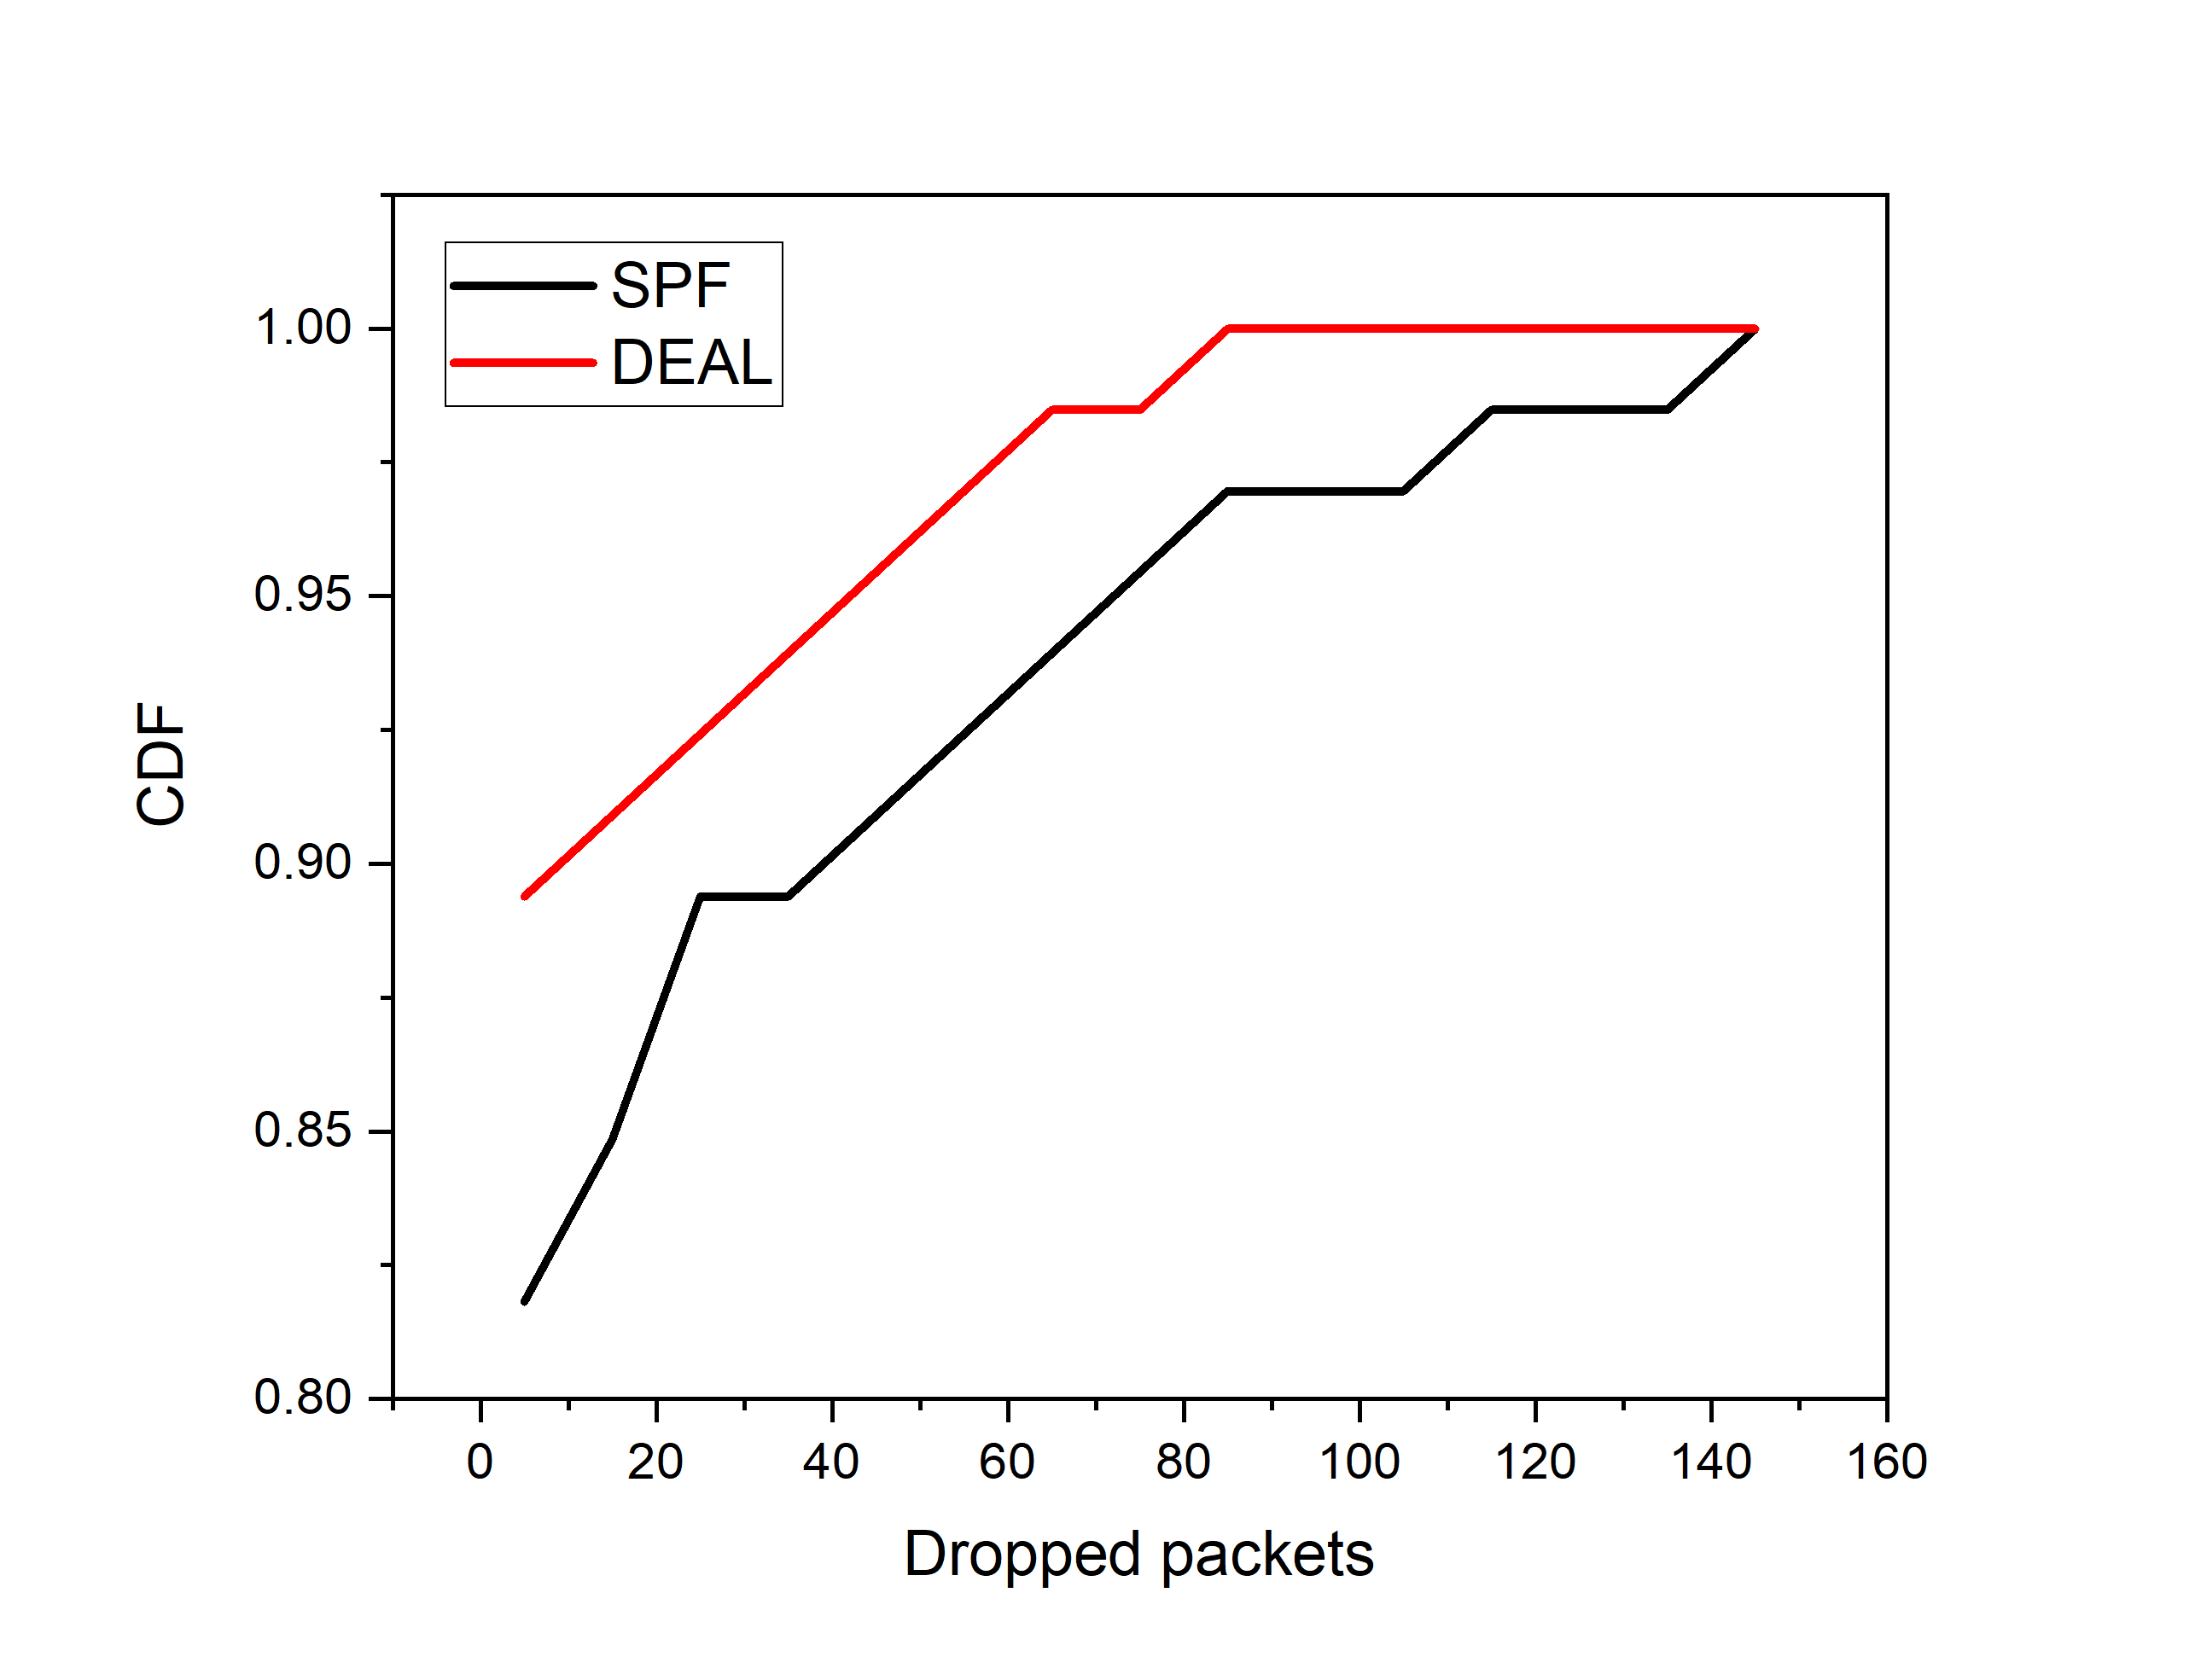
\includegraphics[width=.8\linewidth]{fig/simulation/droppedpacket/DroppedPacketsCDF.png}
		\label{fig:DROPPEDPACKETSCDF}
		}
\caption{ (a) Dropped packets of each satellite (b) CDF of dropped packets}
\label{fig:DROPPED}
\end{figure}

Below in order to compare the link utilization, end-to-end delay, and remaining battery of two schemes under the same delivery ratio.  We set the higher channel data rate and larger queue size as 15Mbps and 650 packet length. When the delivery ratios of the two schemes are different, the impact of undelivered packets can  not be evaluated fairly.


\subsection{Impact of Battery}
At first, we compare the remaining battery energy of the two schemes. In \ref{fig:SPFENERGY} and  \ref{fig:DEALENERGY}, the remaining energy of each satellite's battery in SPF is more diverse than that of DEAL. The standard deviation of remaining energy in SPF is 1127.5, and the standard deviation of remaining energy in DEAL is 1020.76. Besides, the minimal remaining energy of SPF, 30.9,  is much smaller than that of DEAL, 59.2, which indicates that the DEAL algorithm outperforms the SPF algorithm bases its routing strategy on only finding one path.  \ref{fig:CDFENERGY} shows the remaining energy CDF of two schemes. Then we can see DEAL can perform better in energy average for satellite networks.

\begin{figure}[htp]
	\centering
	\subfigure[]{
		\centering
		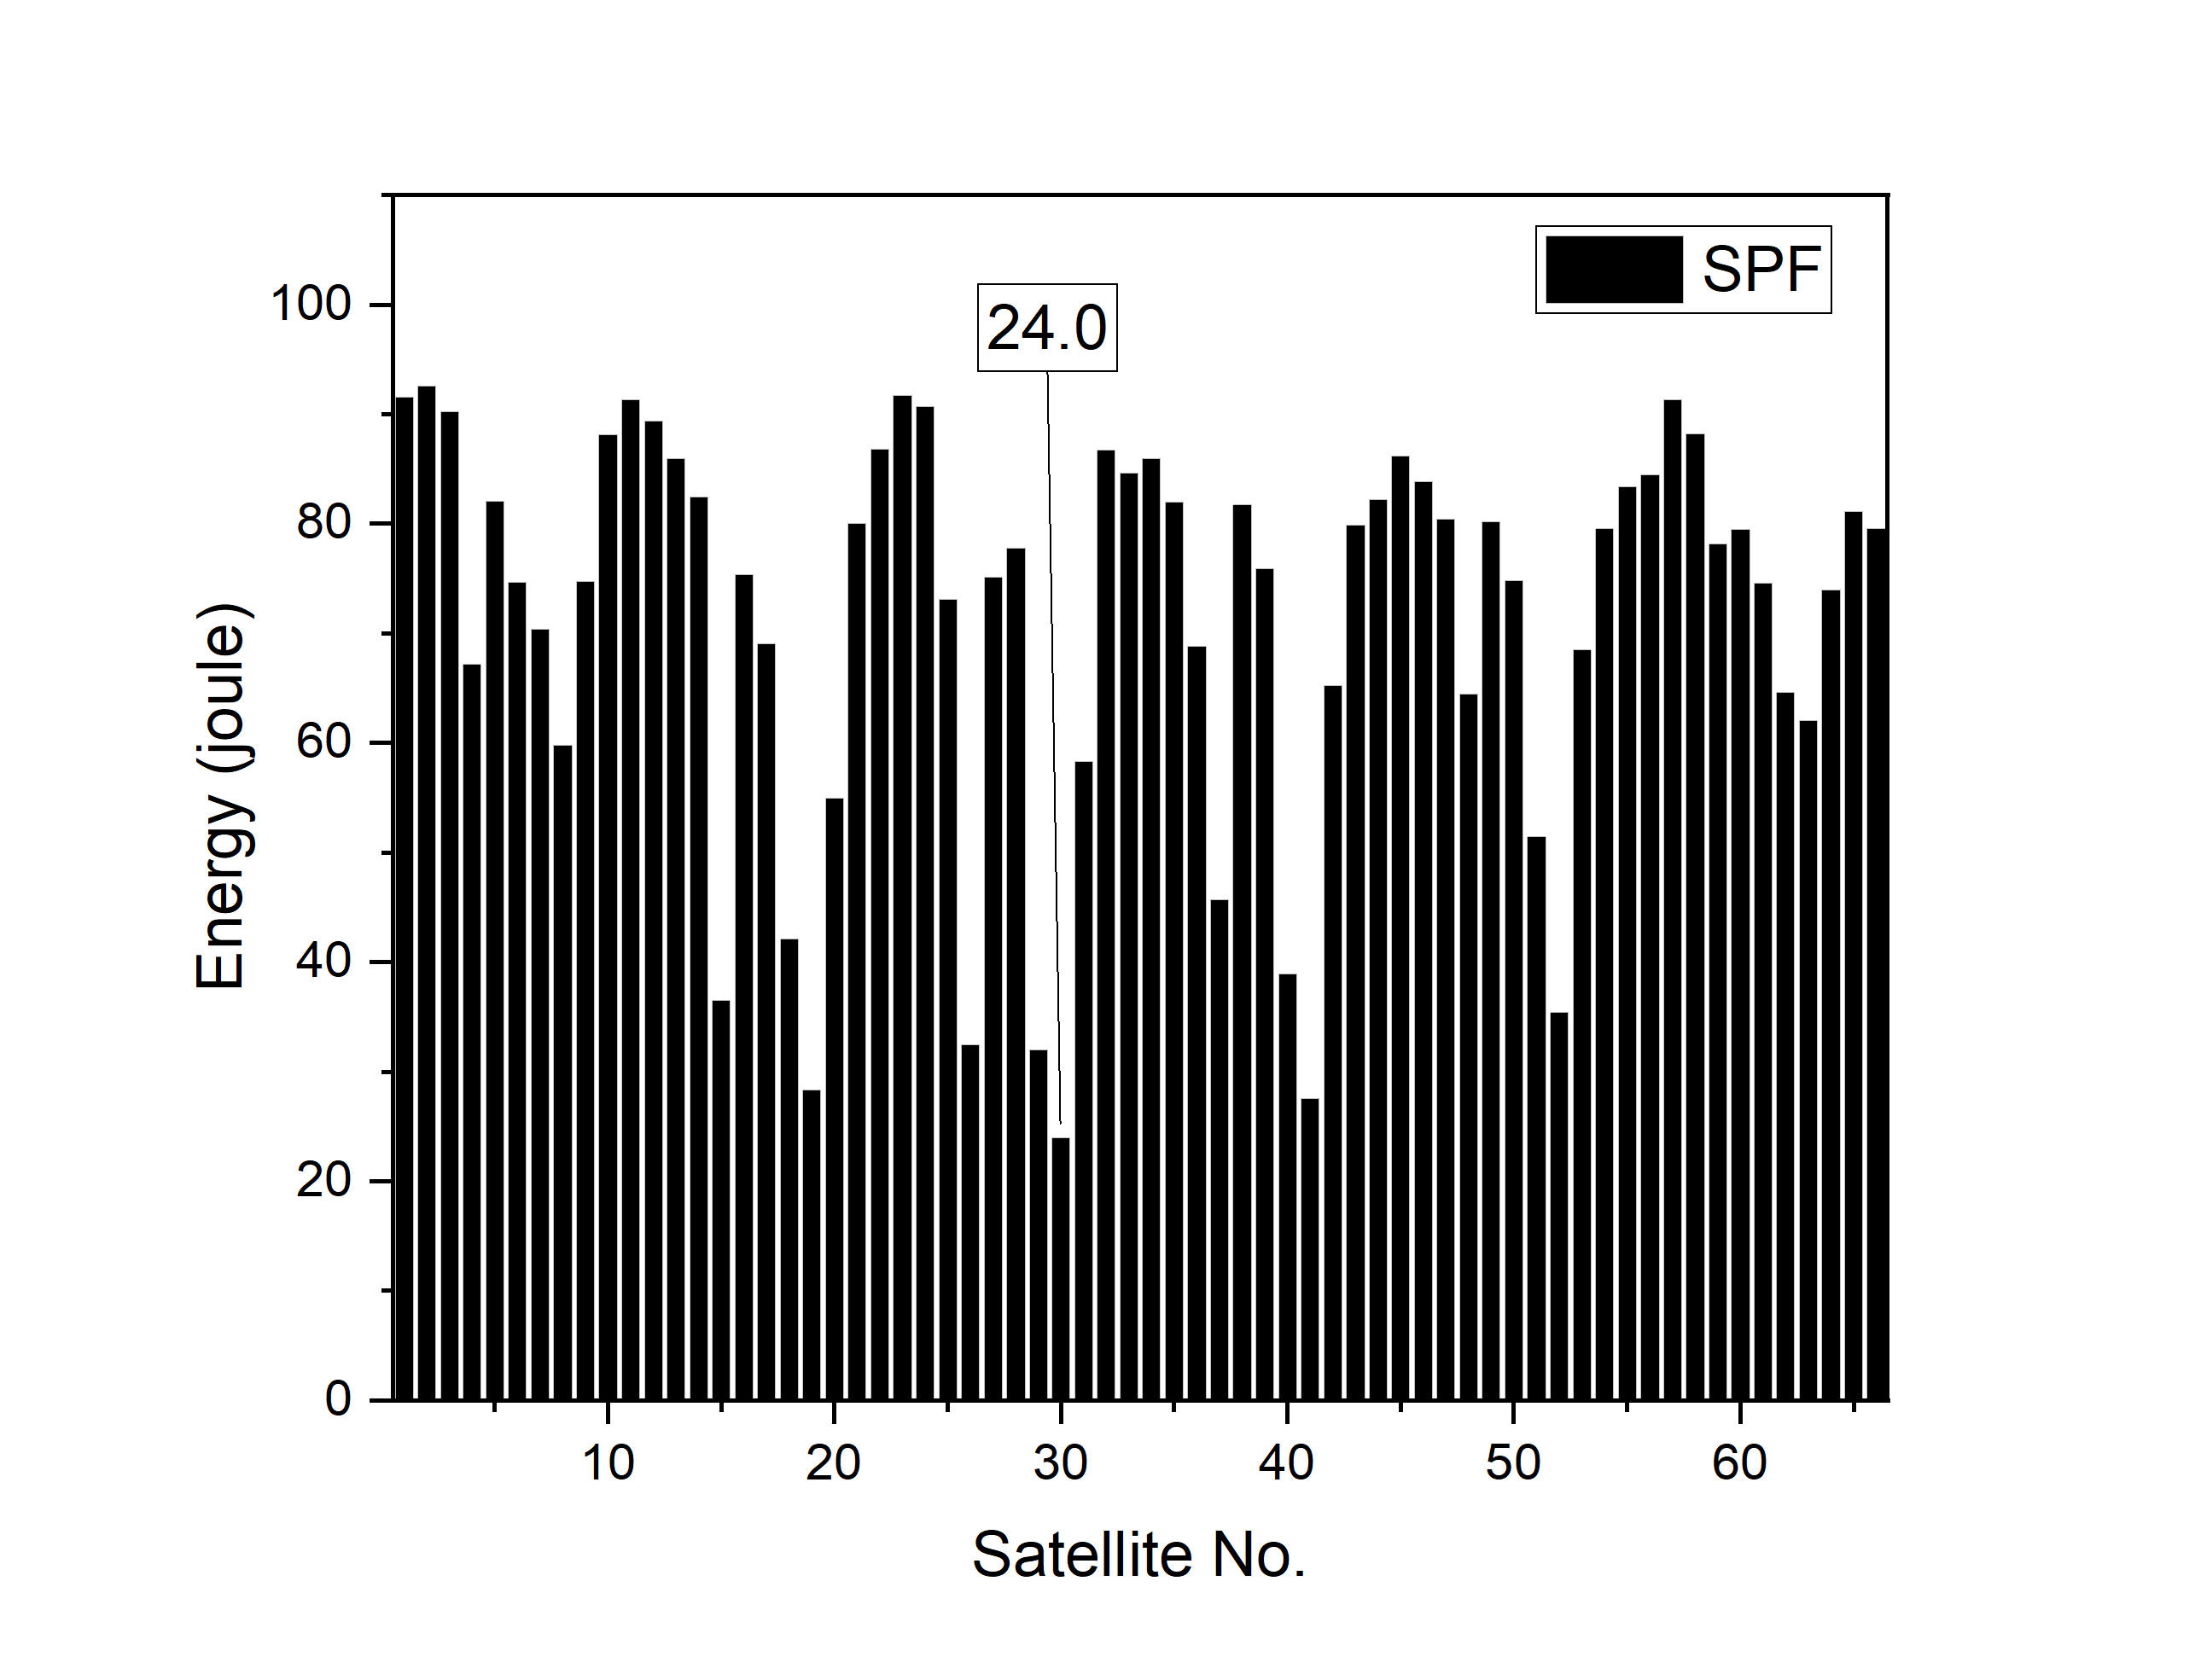
\includegraphics[width=.8\linewidth]{fig/simulation/energy/SPF-ENERGY.png}
		\label{fig:SPFENERGY}
		}
	\subfigure[]{
		\centering
		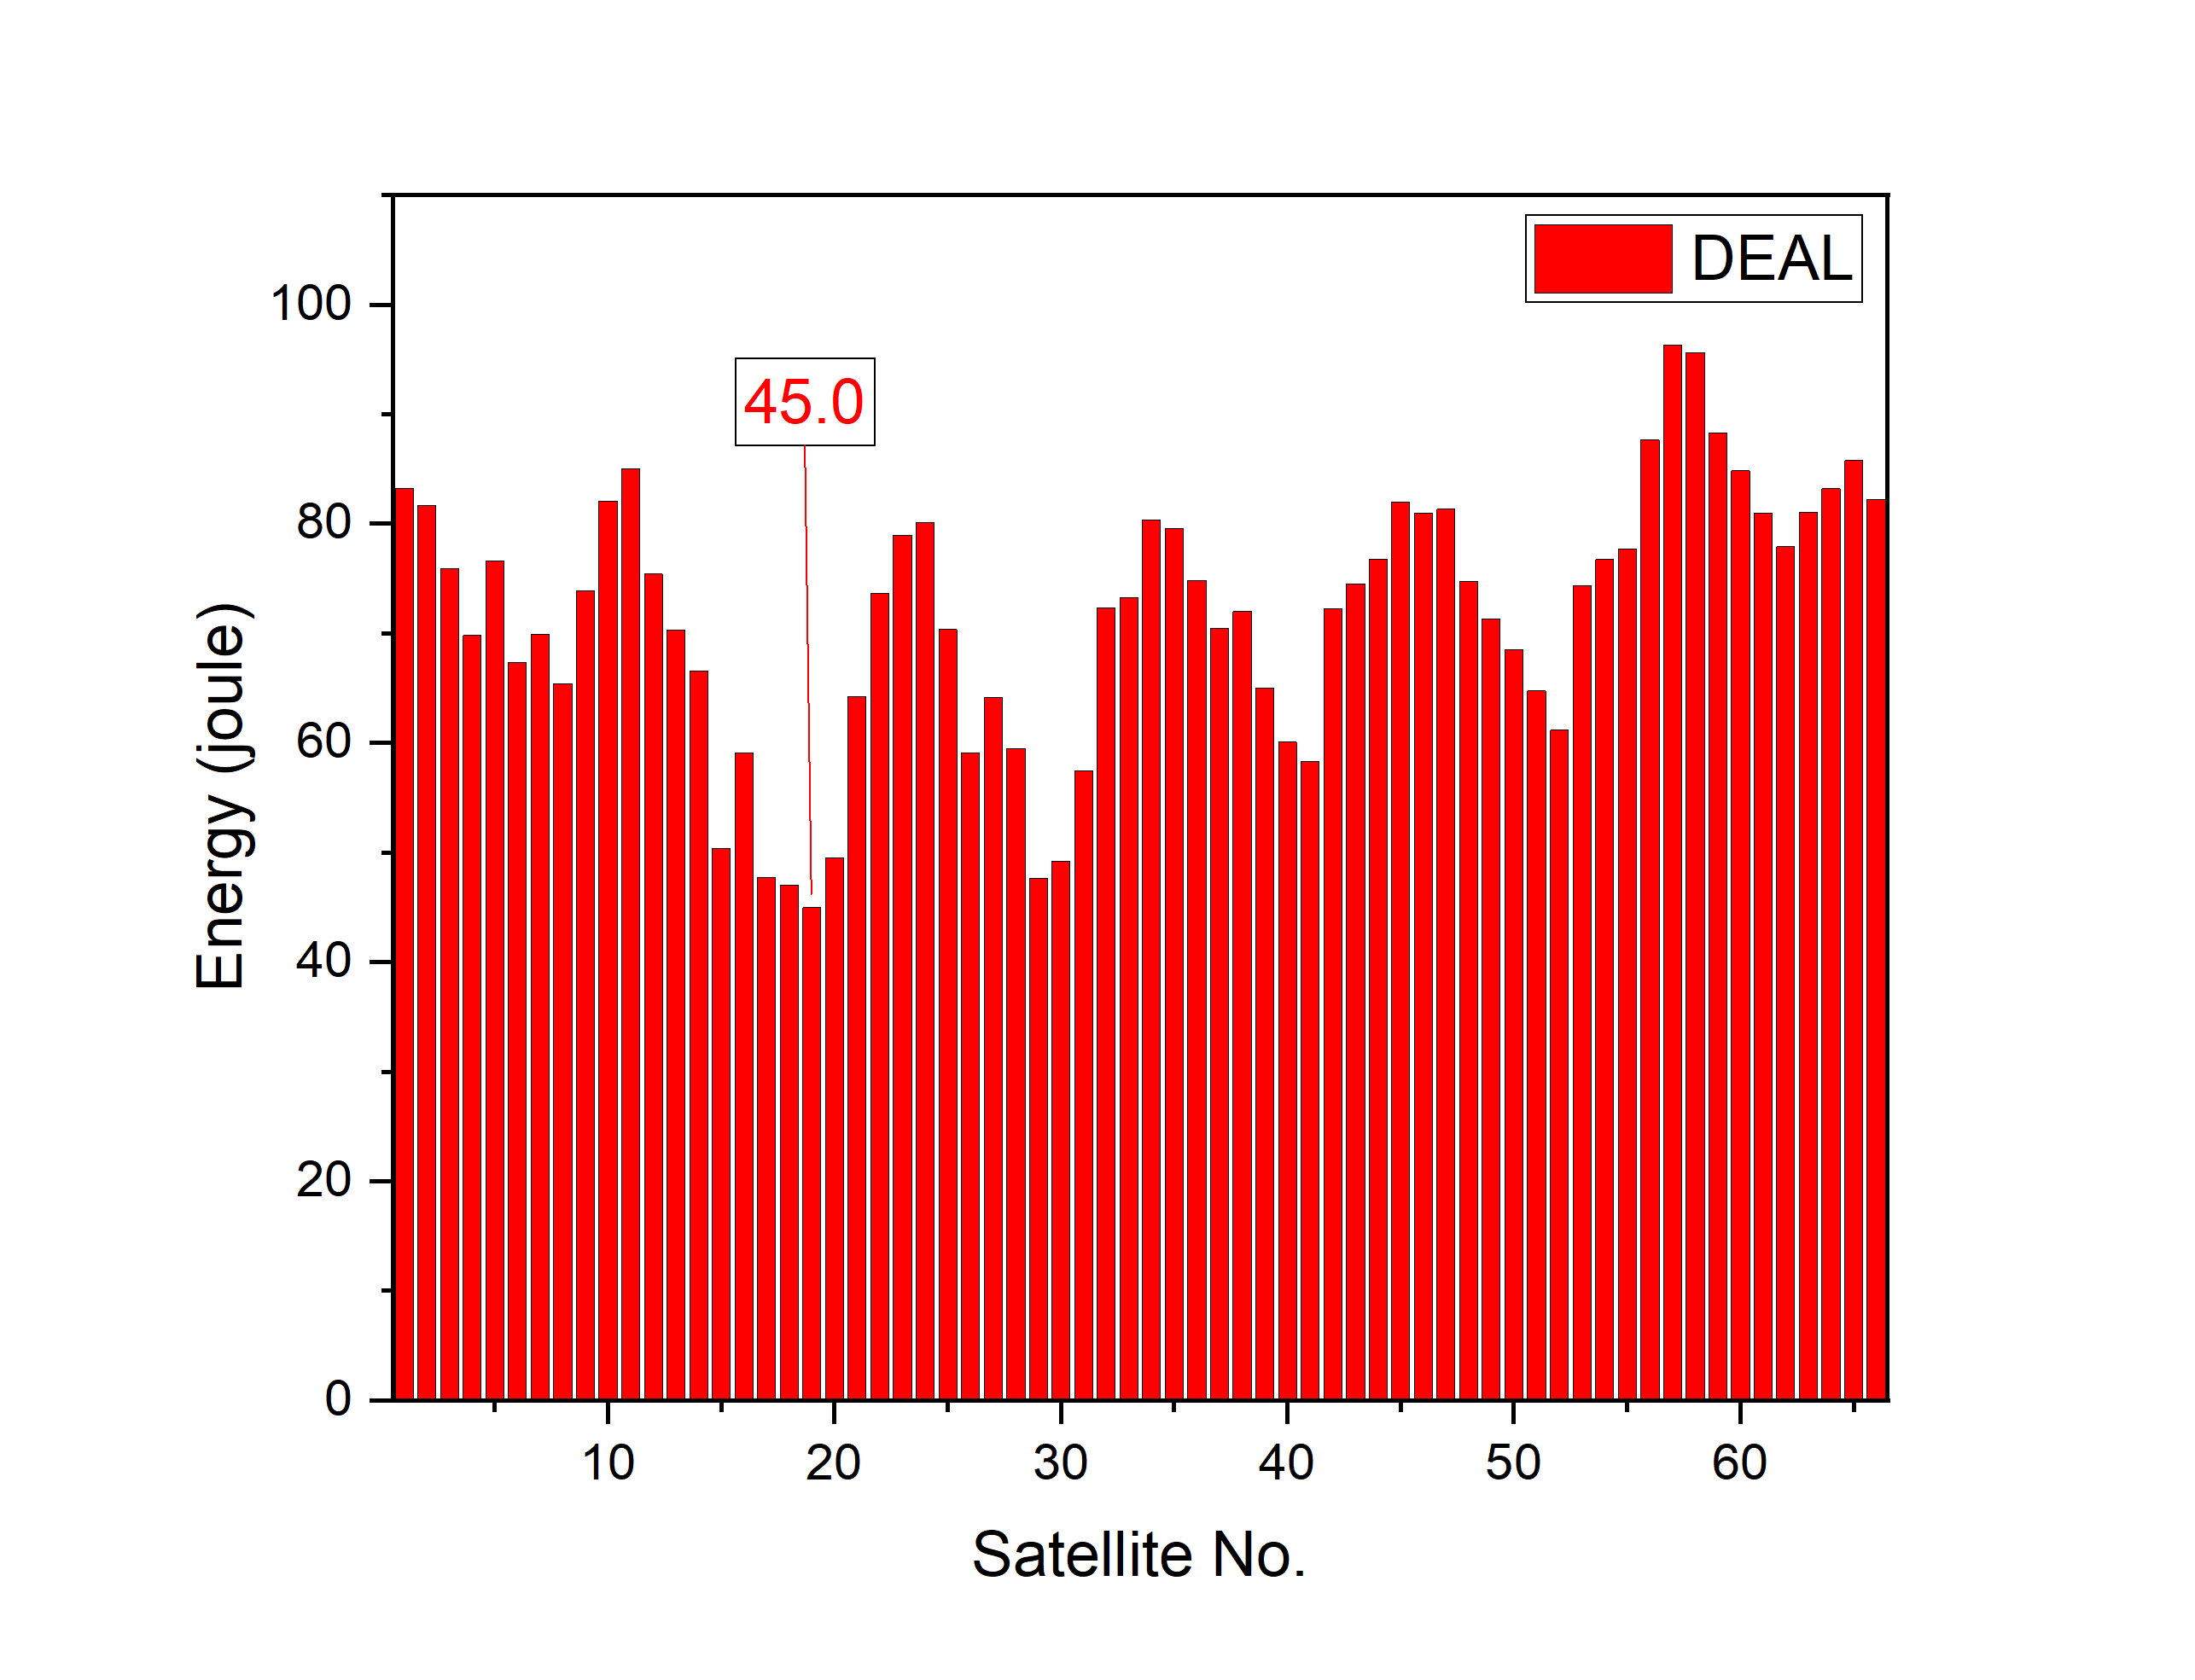
\includegraphics[width=.8\linewidth]{fig/simulation/energy/DEAL-ENERGY.png}
		\label{fig:DEALENERGY}
		}
	\subfigure[]{
		\centering
		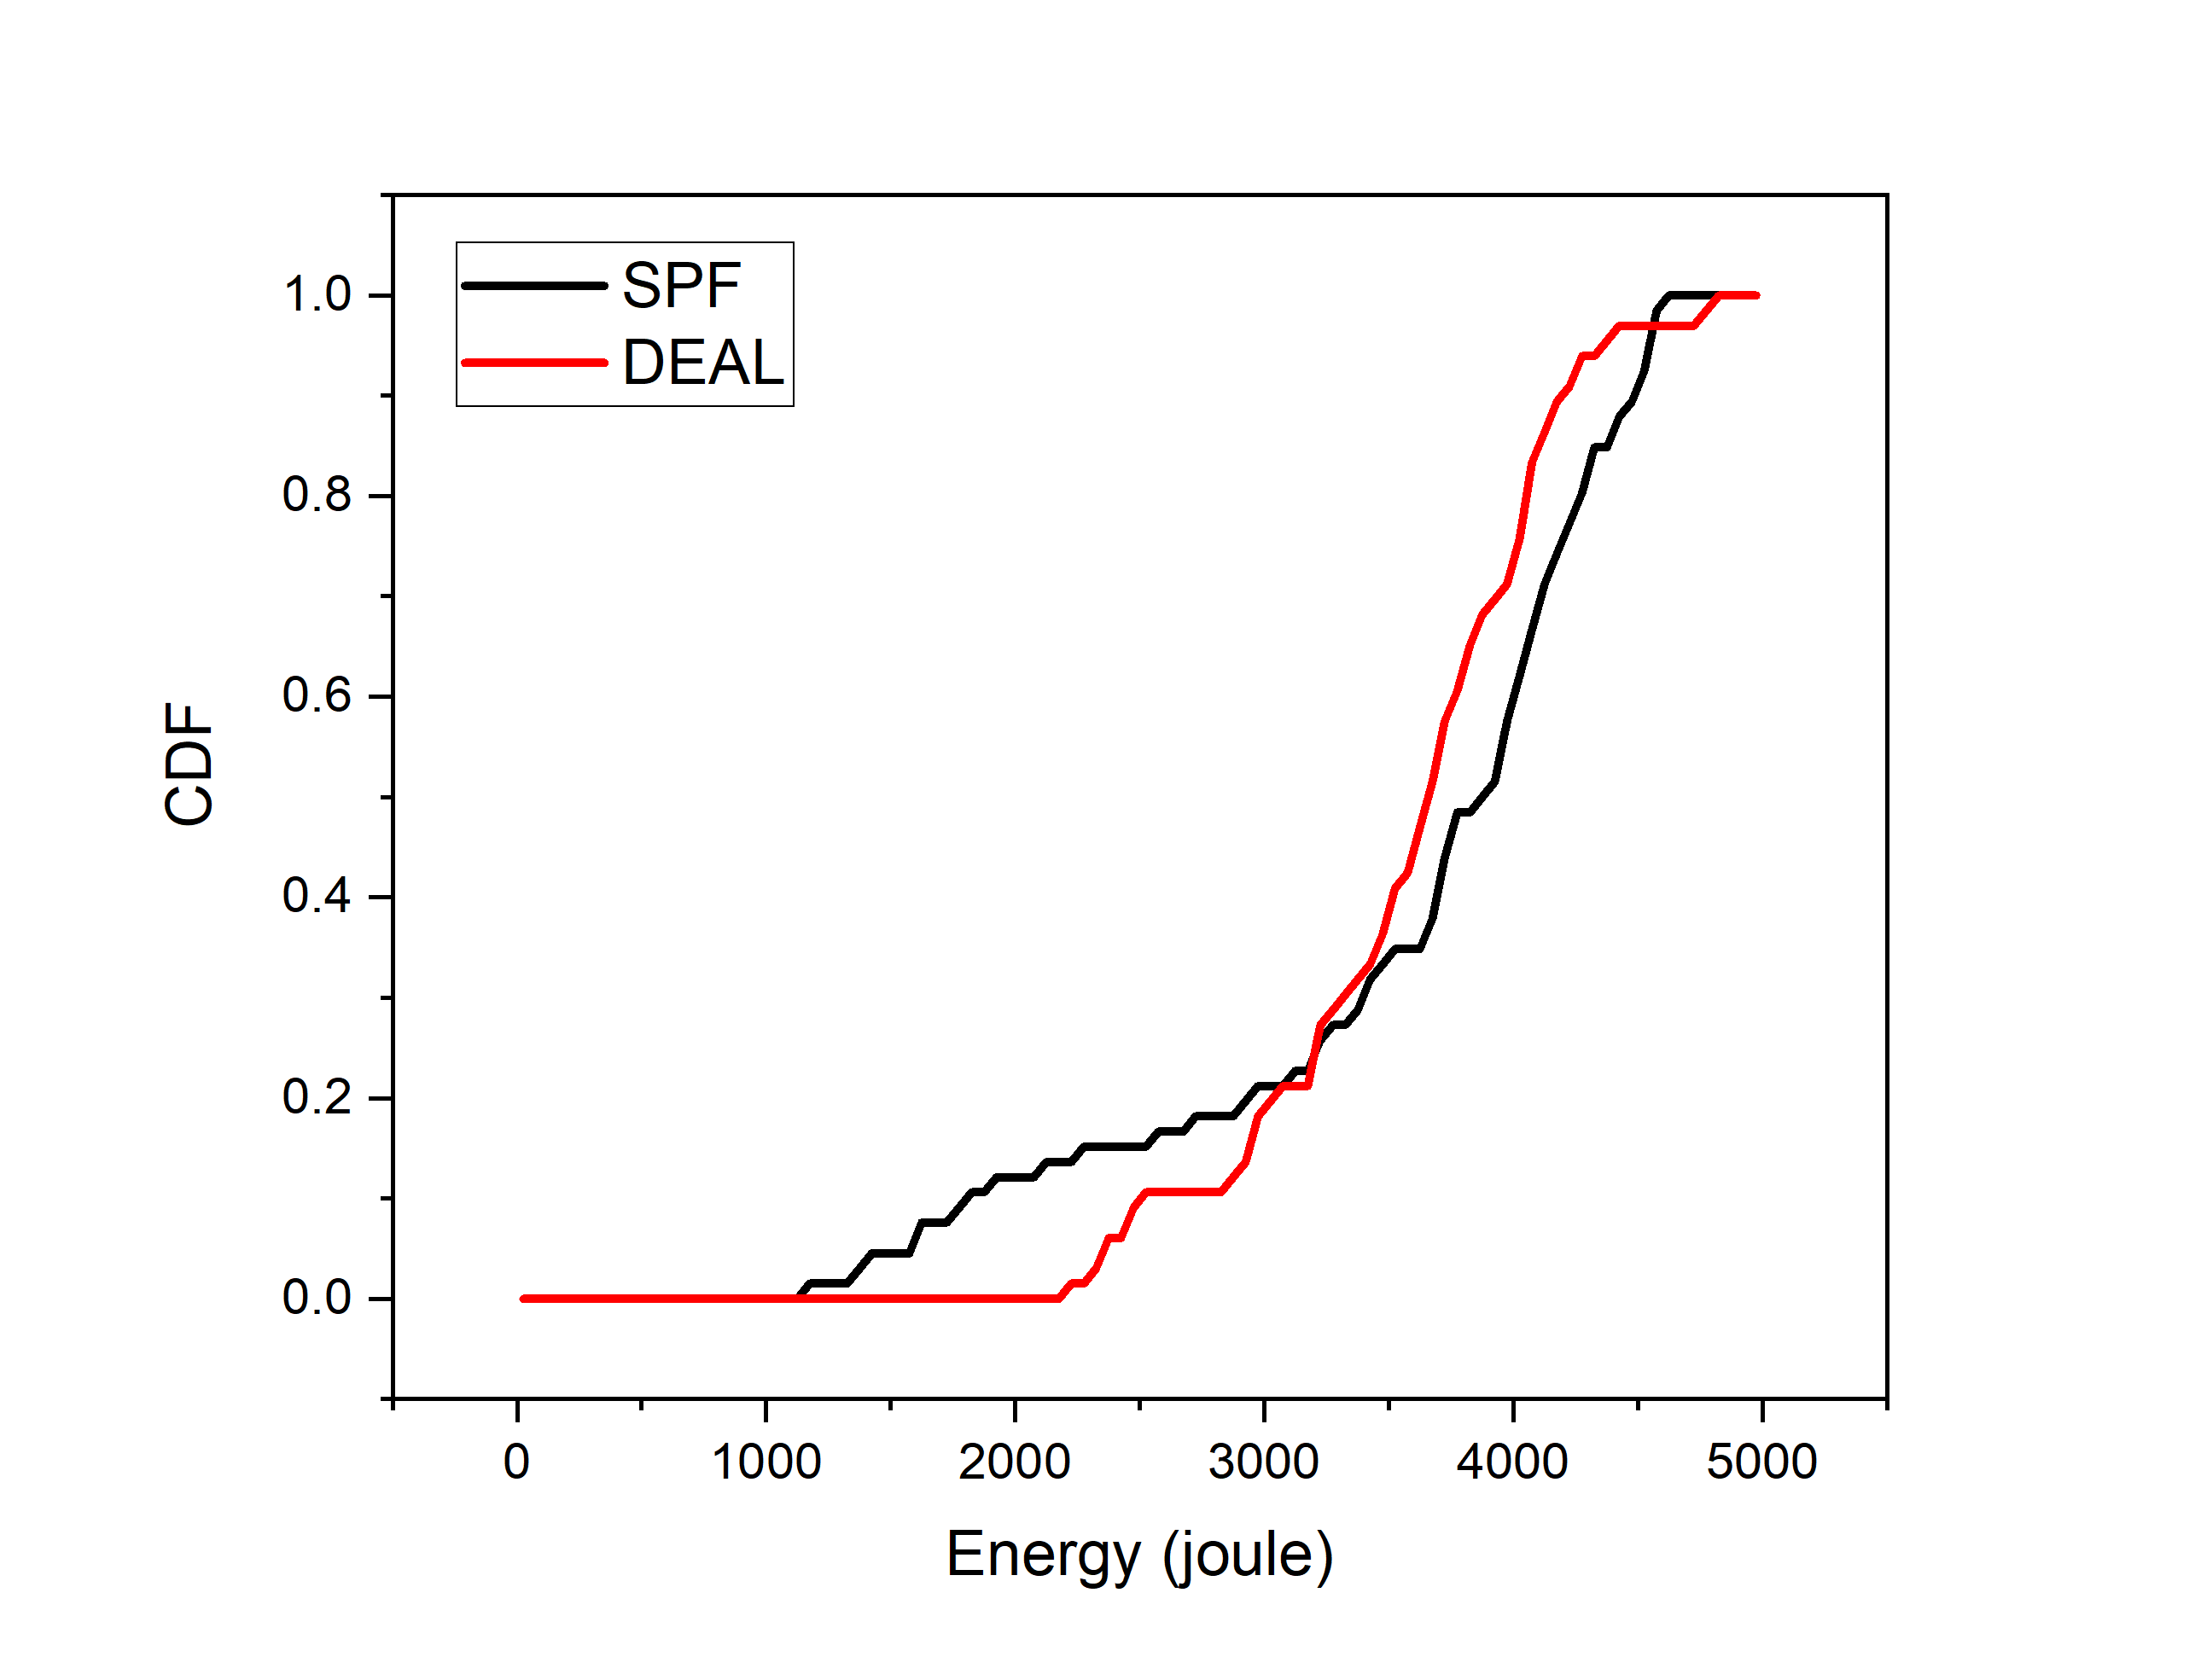
\includegraphics[width=.8\linewidth]{fig/simulation/energy/CDF-ENERGY.png}
		\label{fig:CDFENERGY}
		}
\caption{ (a) Remaining energy of each satellite in SPF (b)  Remaining energy of each satellite in DEAL (c) CDF of remaining energy}
\label{fig:ENERGY}
\end{figure}

\subsection{Impact of Link Utilization}
\ref{fig:LU} shows the link utilization. All the links in satellite constellation are labelled as 3-digit number. Compared to SPF, our DEAL has smaller link utilization, most link has utilization lower than 25\%. Moreover, SPF's mean link utilization is about 0.080202, while DEAL's mean value of link utilization is about 0.0731. The standard deviation of SPF is 0.06606, and DEAL's is 0.0549, and the CDF of link utilization is shown in \ref{fig:LUCDF}. The highest link utilization in SPF is 32.76563, while the highest one in DEAL is 27.5531. This is because DEAL splits the flows and reduces the possiblity of congestion.

\begin{figure}[htp]
	\subfigure[]{
		\centering
		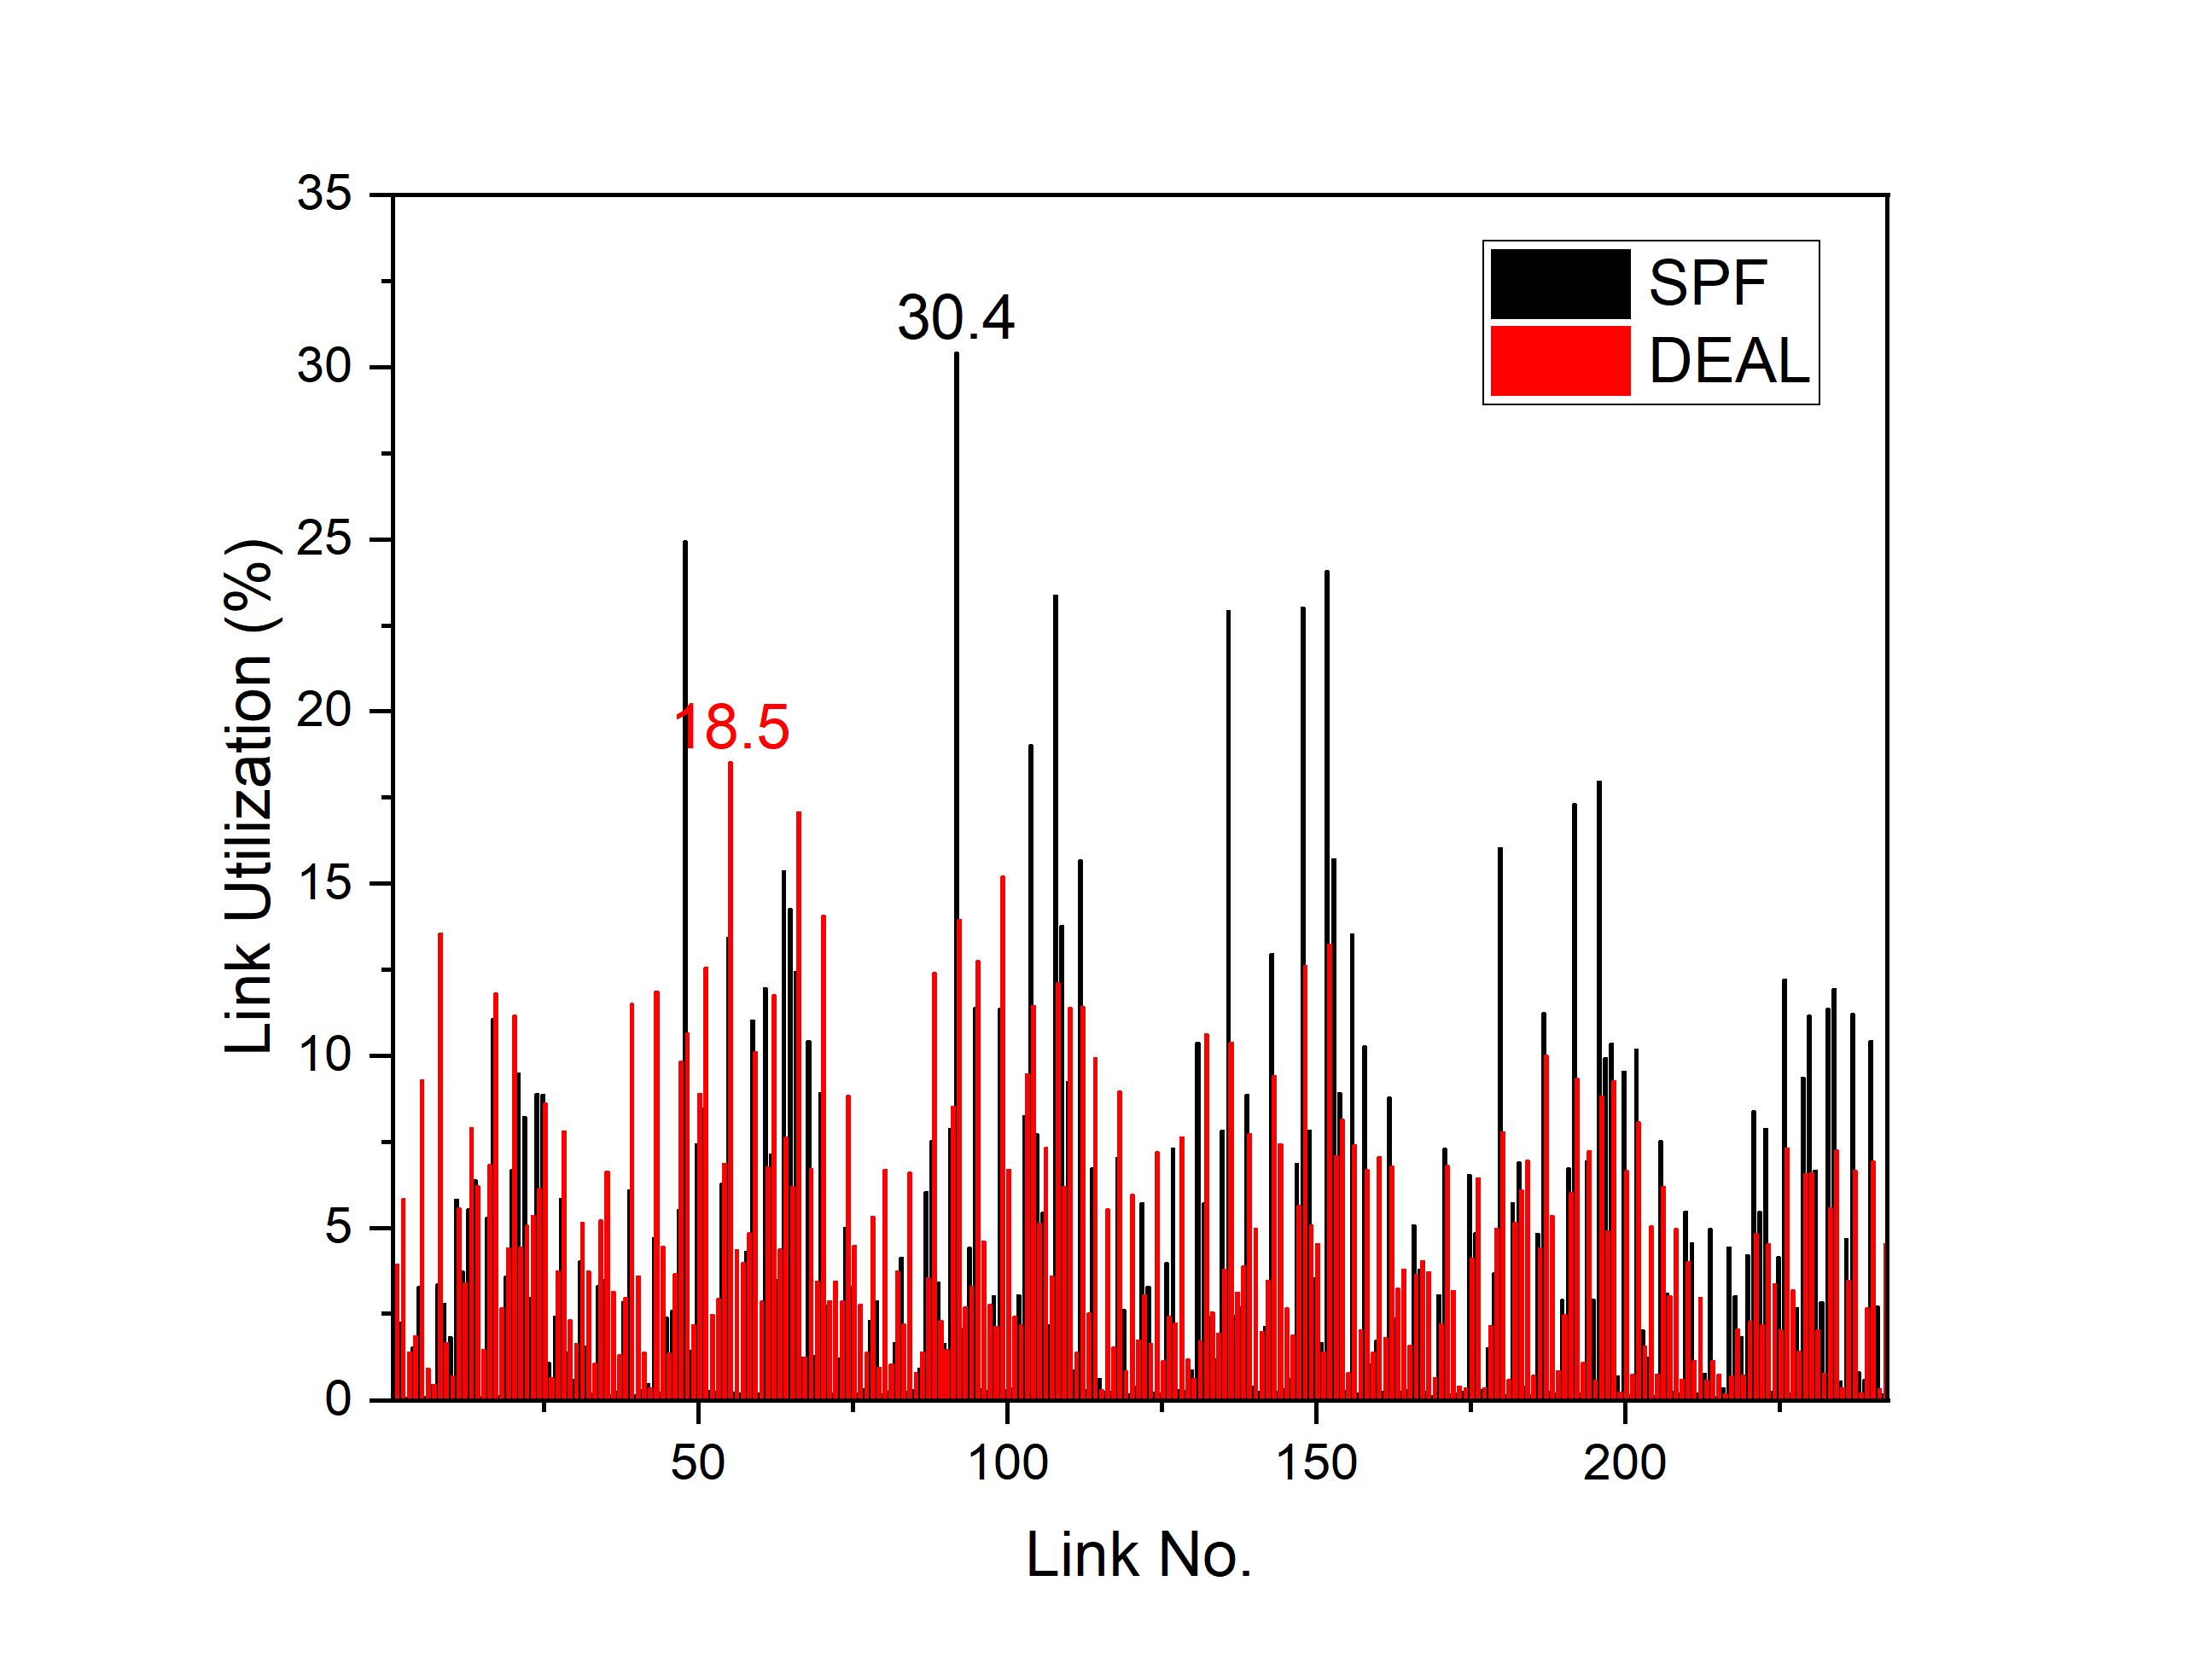
\includegraphics[width=.8\linewidth]{fig/simulation/linkUtilization/LinkUtilization.png}
		\label{fig:LU}
		}
	\subfigure[]{
		\centering
		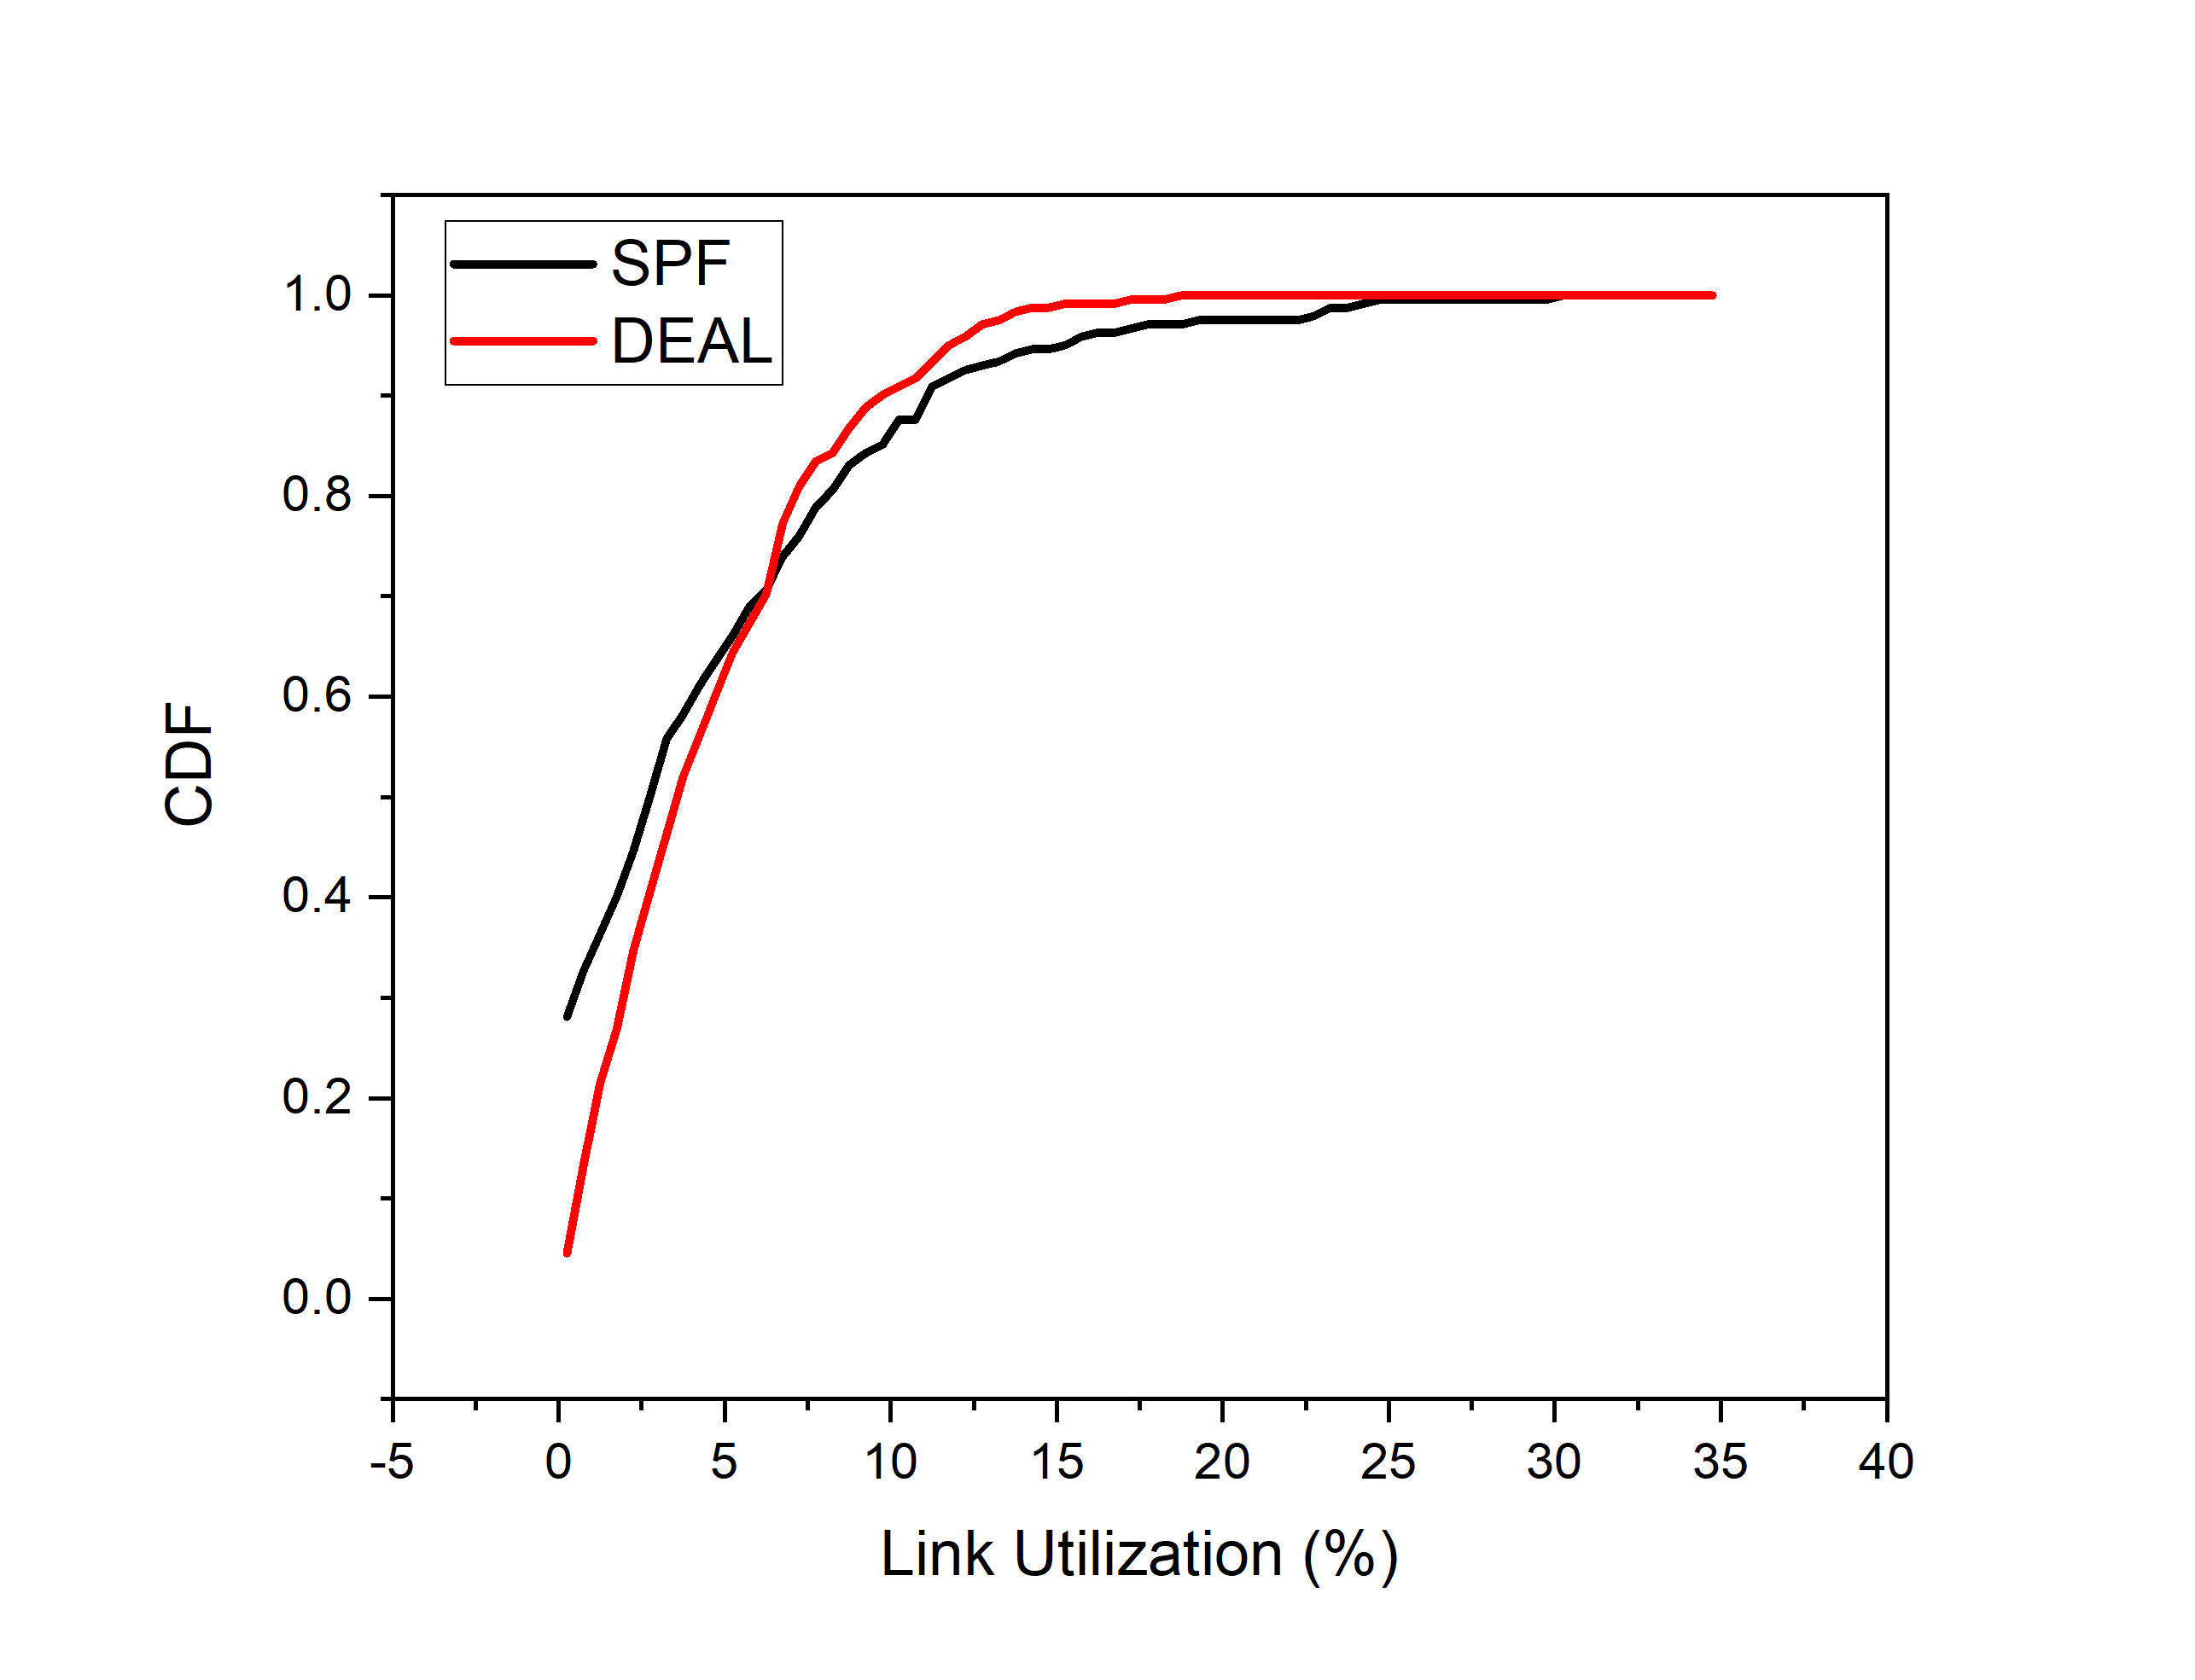
\includegraphics[width=.8\linewidth]{fig/simulation/linkUtilization/LinkUtilizationCDF.png}
		\label{fig:LUCDF}
		}
	
\caption{(a) Link utilization of each link (b) CDF of link Utilization}
\label{fig:UTILIZATION}
\end{figure}


\subsection{Impact of End-to-End Delay }

The mean end-to-end delay of a satellite is the average delay of packets of the same communication satellite pair. In our simulation, the mean delay of a packet in SPF is about 0.153ms, and the mean delay of a packet in DEAL is about 0.136ms. The mean delay of each satellite is presented in \ref{fig:ENDTOENDDELAY}. in which the average delay is calculated and presented.  The two schemes have a slight difference which comes from the queuing delay.

\begin{figure}[htp]
	\centering
	
	\subfigure[]{
		\centering
		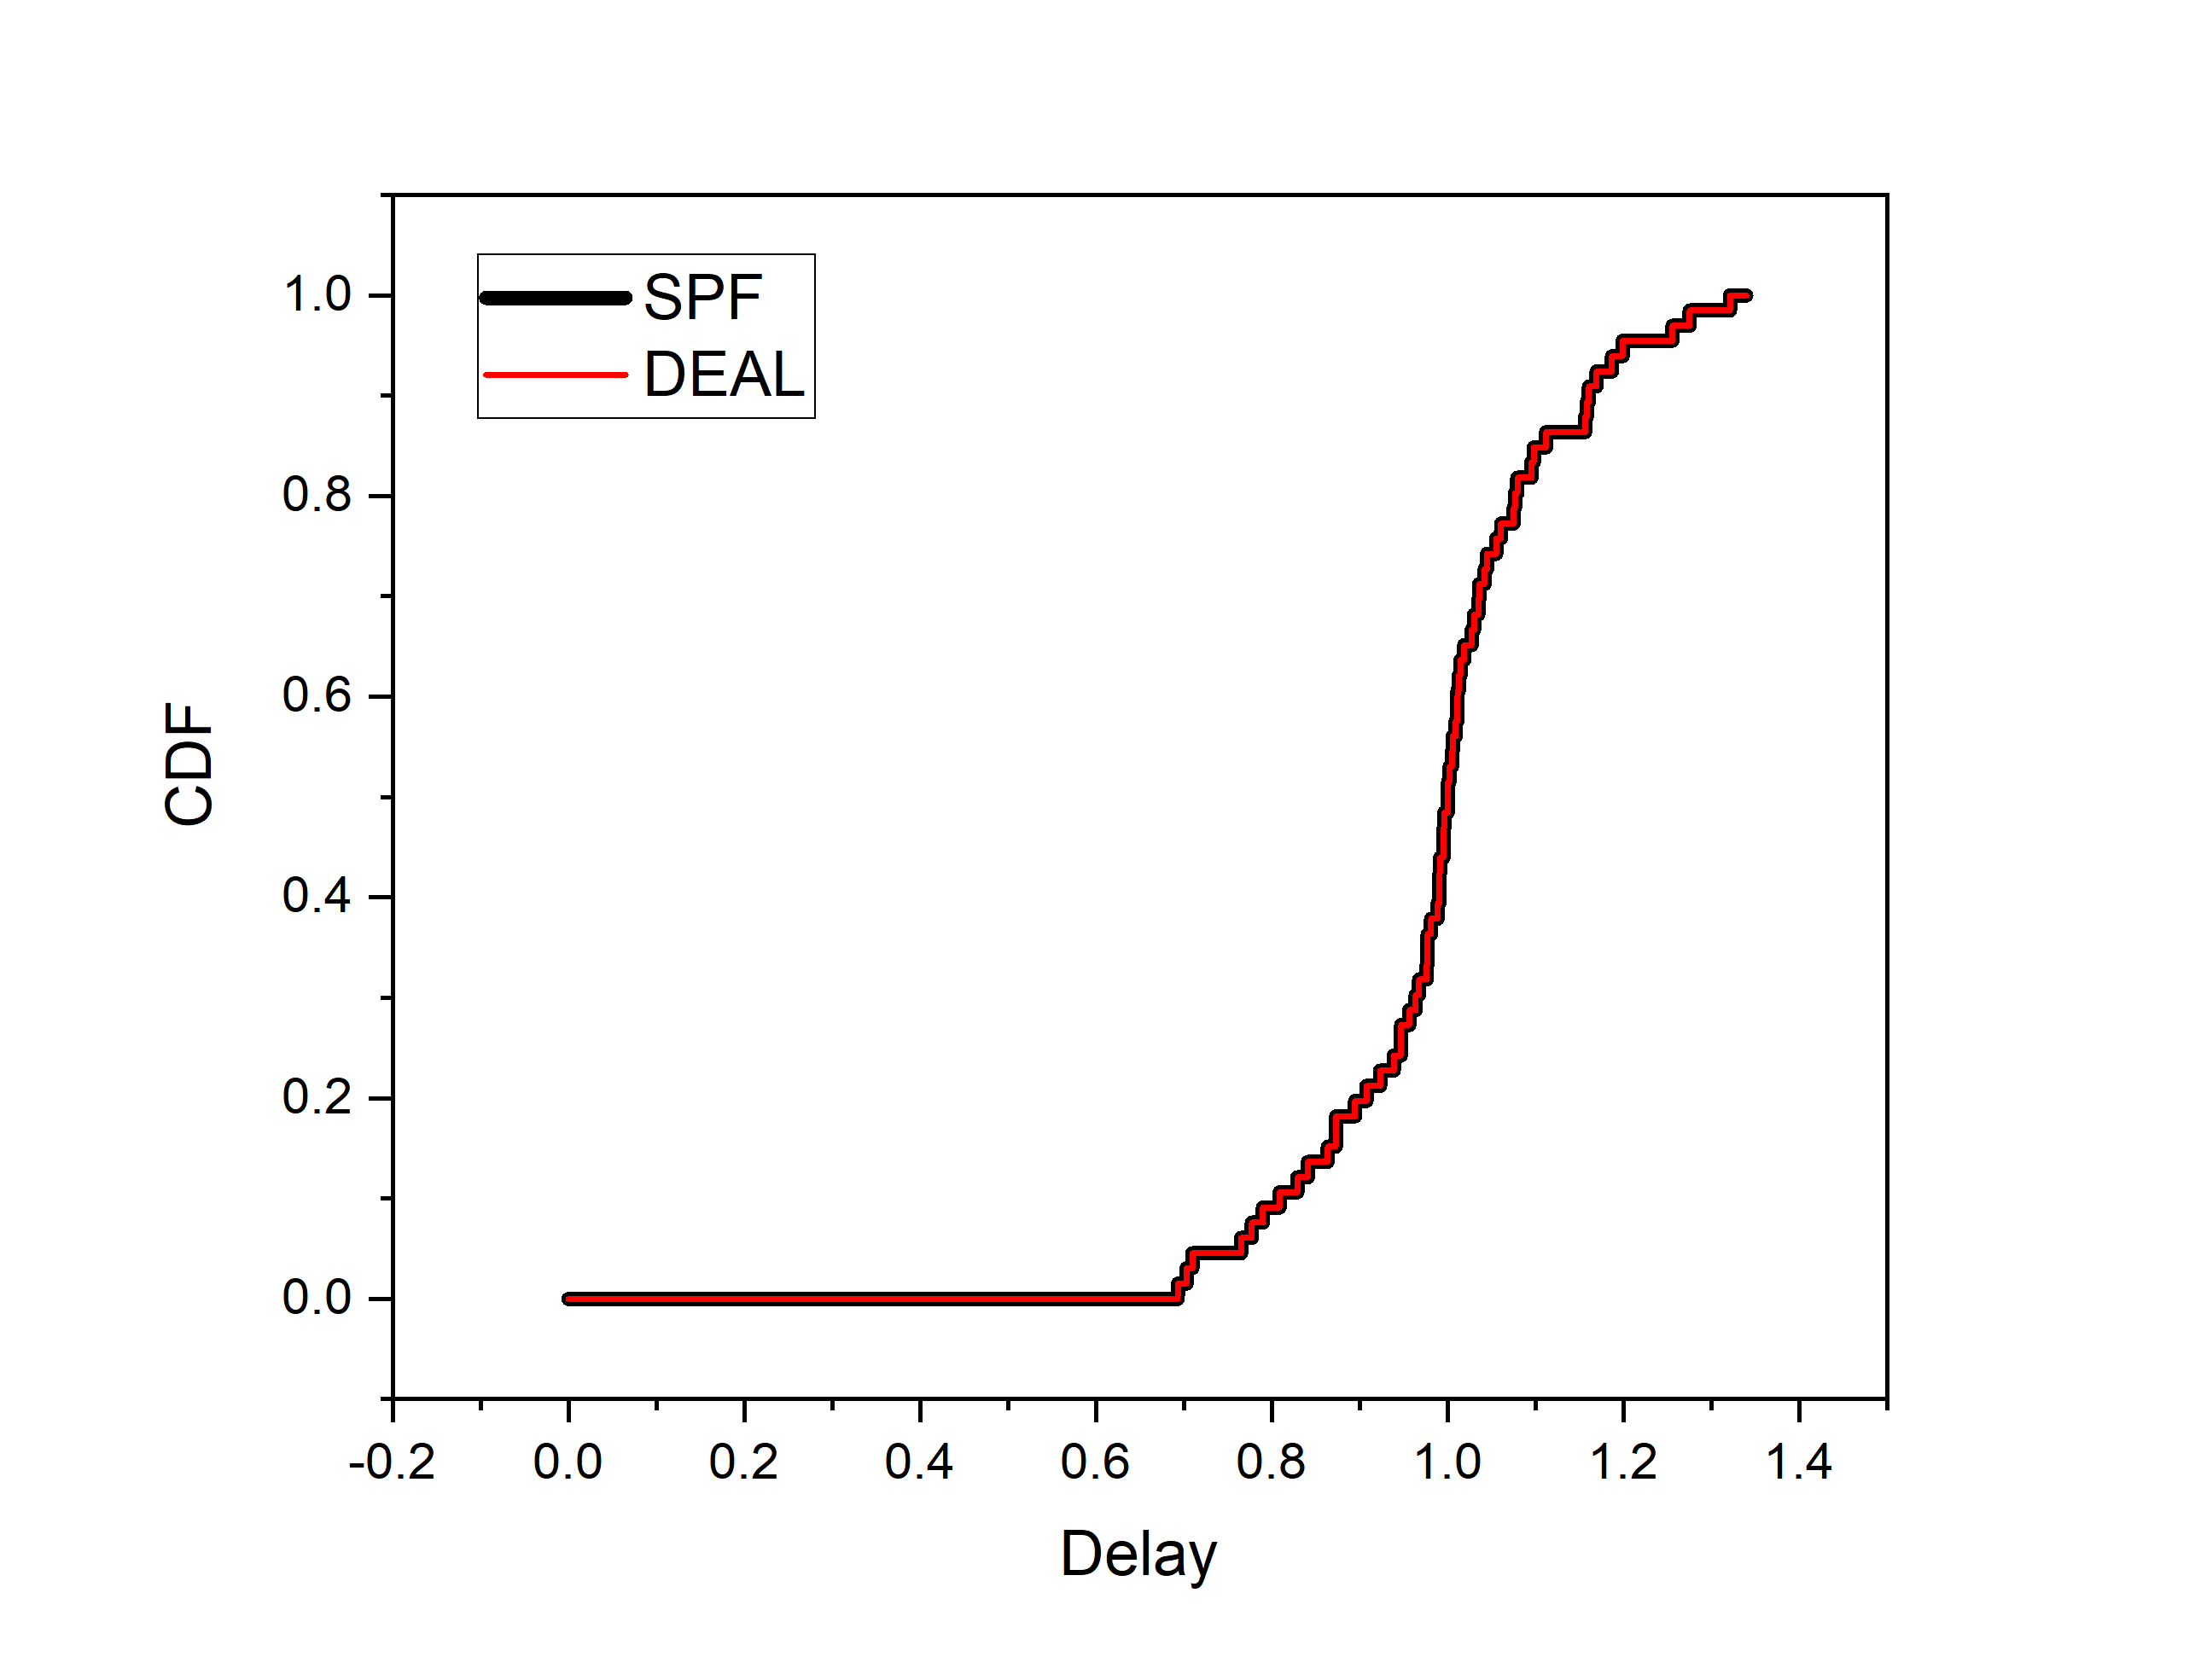
\includegraphics[width=.8\linewidth]{fig/simulation/delay/ENDTOENDDELAY.png}
		\label{fig:ENDTOENDDELAY}
		}
	
\caption{CDF of Mean End-to-End Delay}
\label{fig:DELAY}
\end{figure}

To show the probability of congestion, we  compare their mean occupying ratio of buffer queues. In \ref{fig:ORES} and \ref{fig:CDFOR}, several satellites in SPF has rather high occupying ratio of the queue. Recall that packets with a given source satellite and destination satellite adopt the same route in SPF, and some satellites became hot-spots. Clearly, congestion happens easily when satellites on the paths cover the high-population area.  DEAL adopts flow splitting to avoid the congestion with different cost value along with distance, the probability of congestion in DEAL can be lower. 

\begin{figure}[htp]
	\centering
	\subfigure[]{
		\centering
		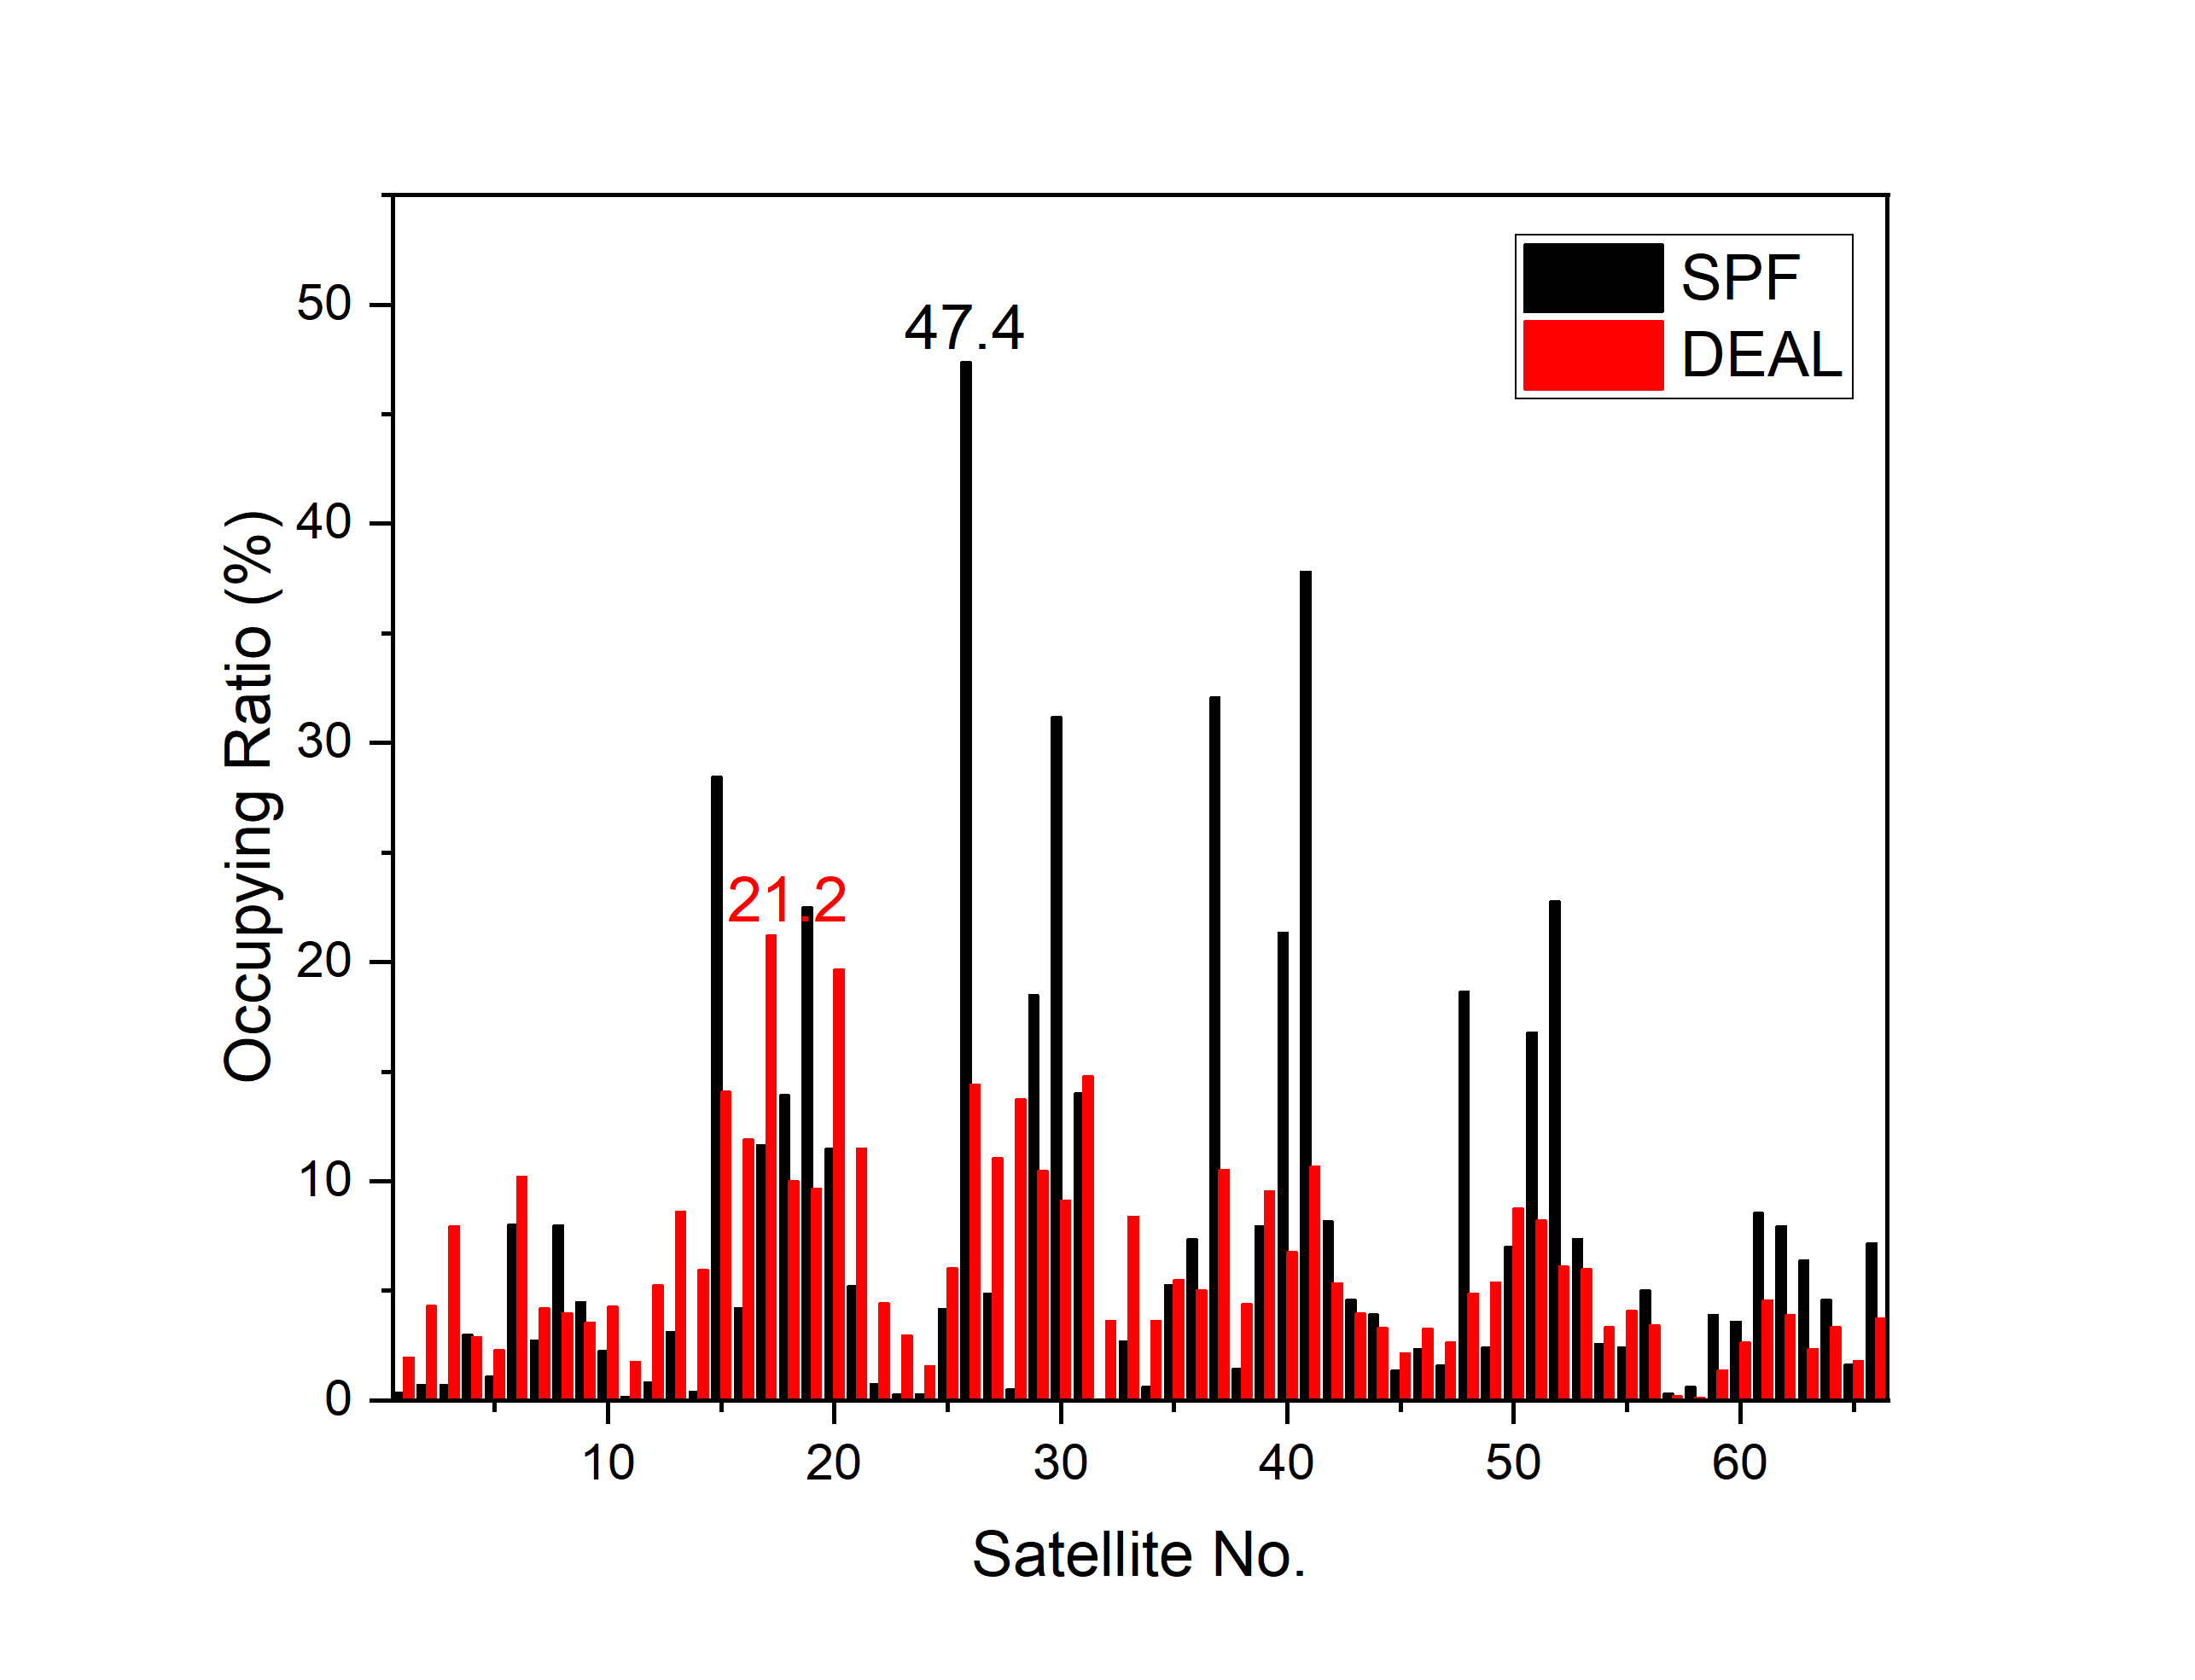
\includegraphics[width=.8\linewidth]{fig/simulation/queue/Occupying ratio of each satellite.png}
		\label{fig:ORES}
		}
	\subfigure[]{
		\centering
		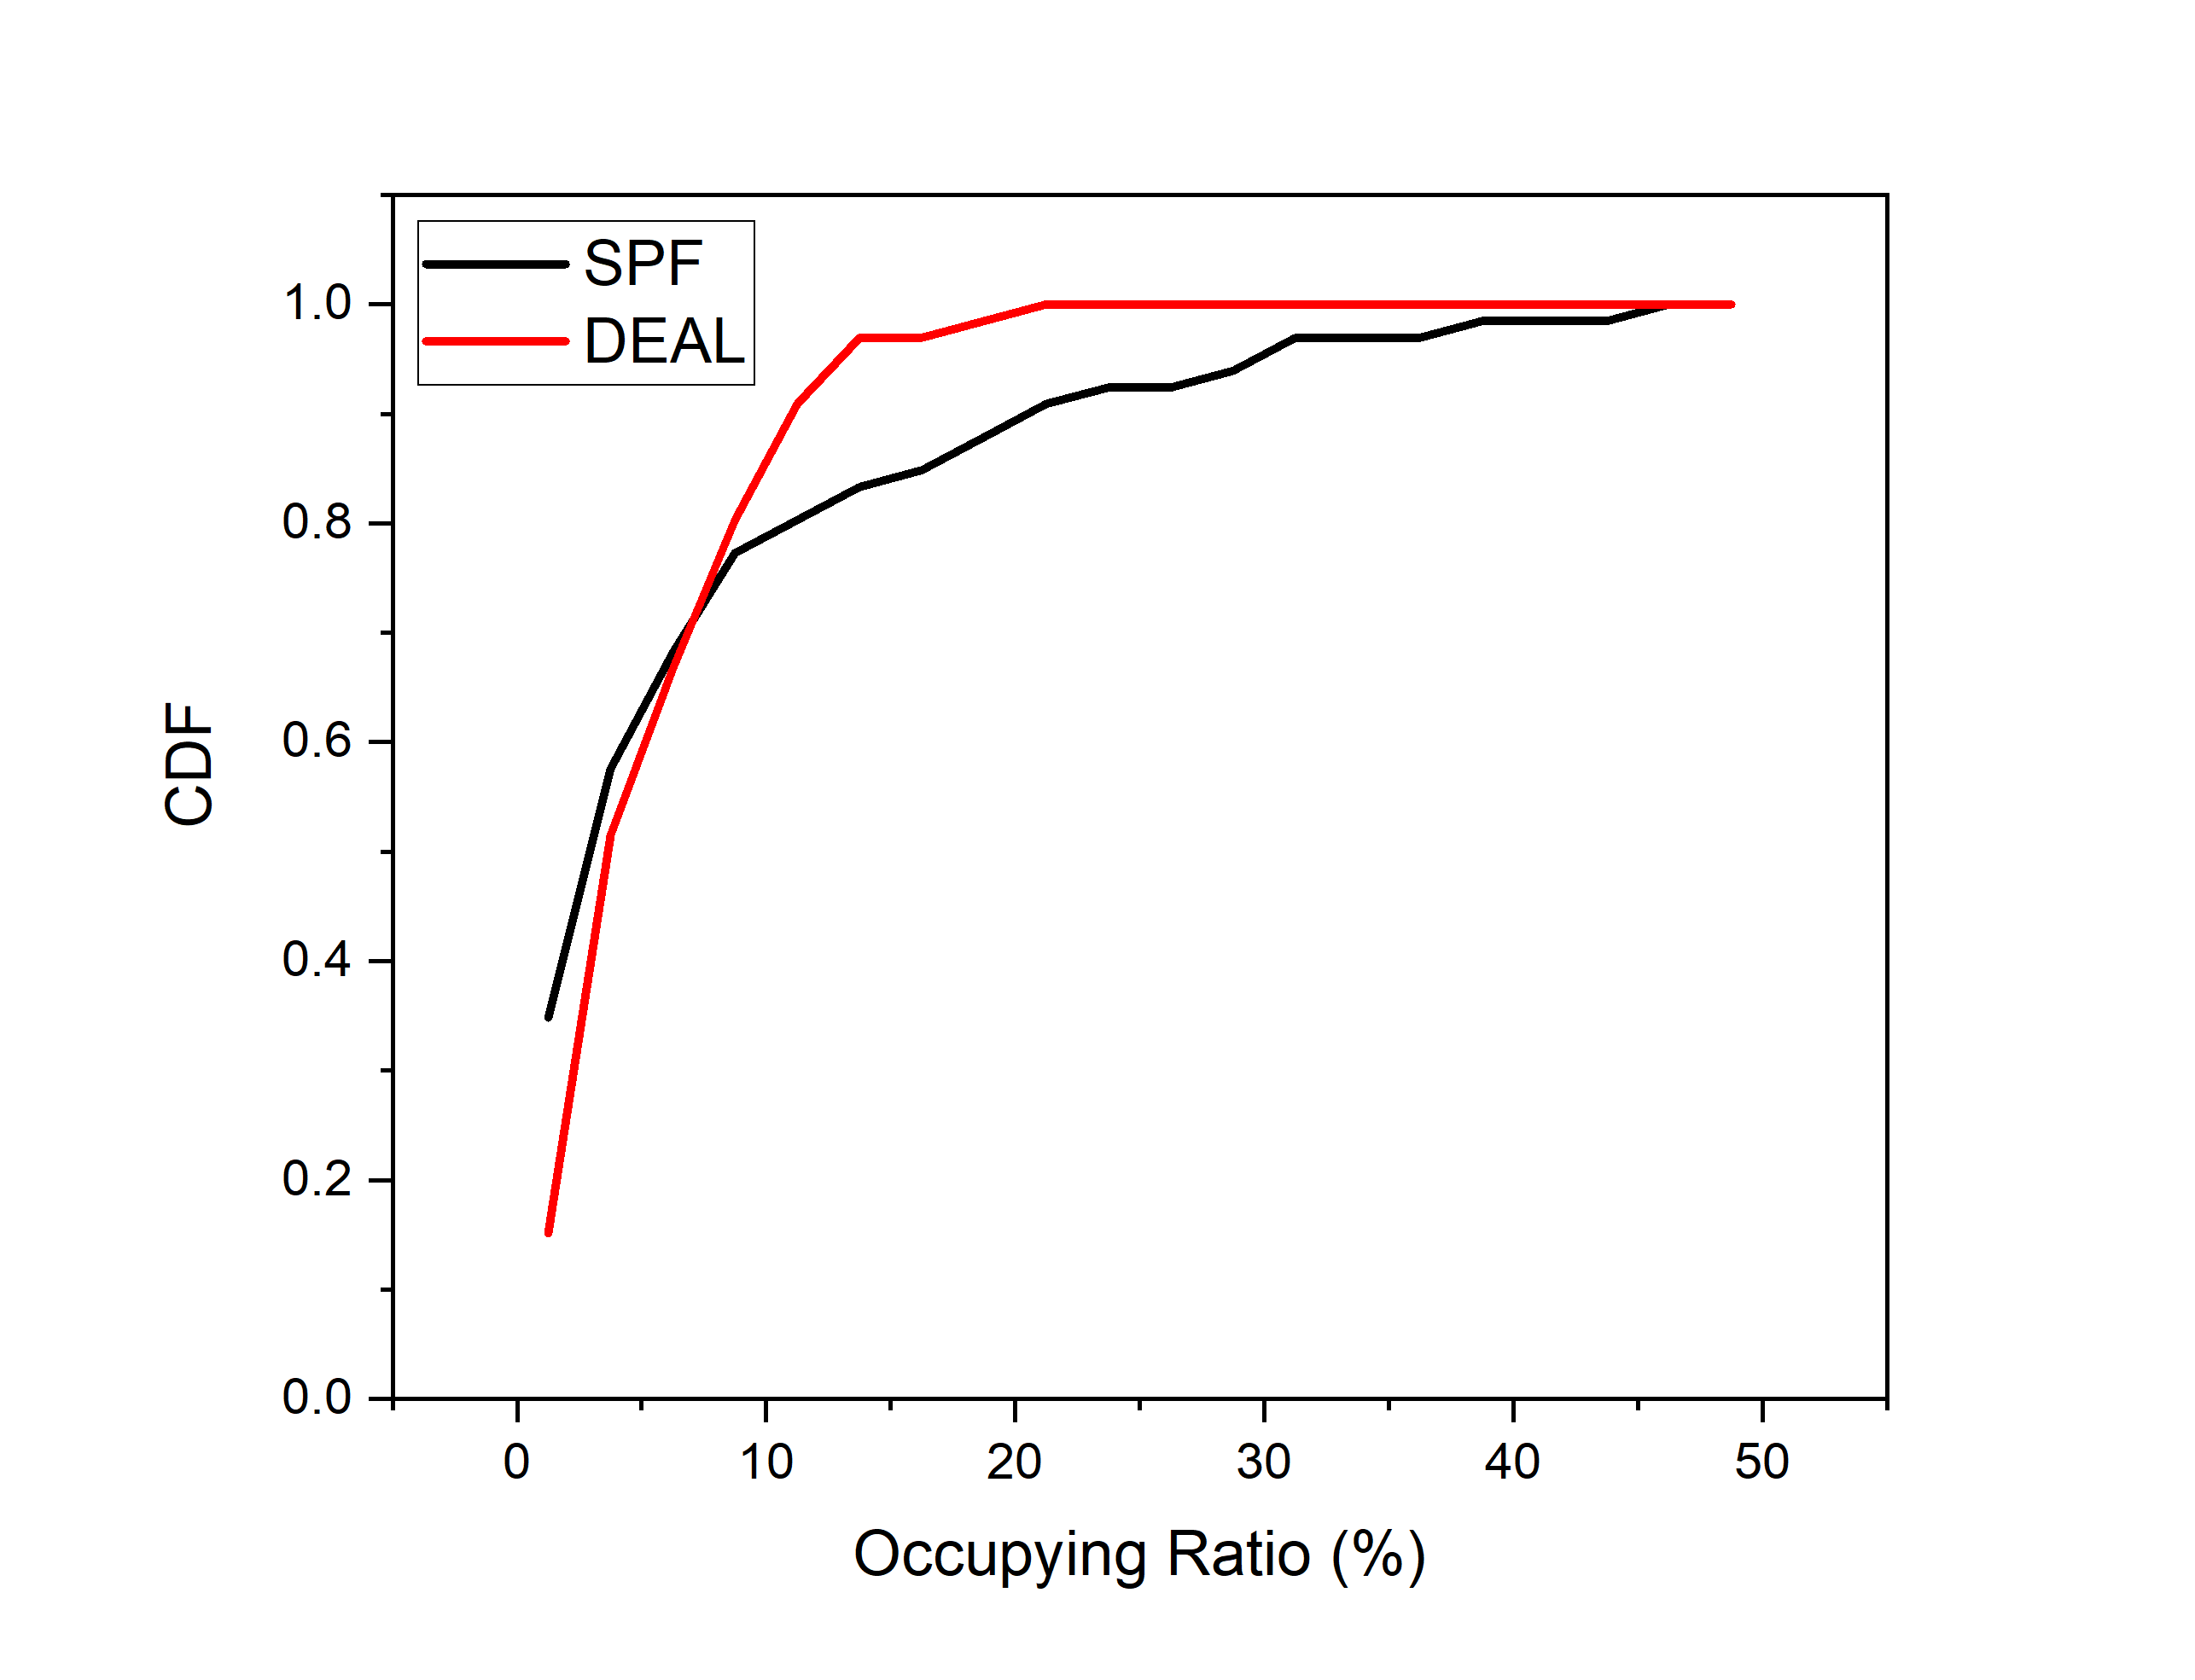
\includegraphics[width=.8\linewidth]{fig/simulation/queue/CDF of Occupying ratio.png}
		\label{fig:CDFOR}
		}
		
\caption{Occupying ratio (a) Ocuppying ratio of each satellite (b) CDF of ocuppying ratio}
\label{fig:OR}
\end{figure}